\documentclass[twoside]{book}

% Packages required by doxygen
\usepackage{fixltx2e}
\usepackage{calc}
\usepackage{doxygen}
\usepackage[export]{adjustbox} % also loads graphicx
\usepackage{graphicx}
\usepackage[utf8]{inputenc}
\usepackage{makeidx}
\usepackage{multicol}
\usepackage{multirow}
\PassOptionsToPackage{warn}{textcomp}
\usepackage{textcomp}
\usepackage[nointegrals]{wasysym}
\usepackage[table]{xcolor}

% Font selection
\usepackage[T1]{fontenc}
\usepackage[scaled=.90]{helvet}
\usepackage{courier}
\usepackage{amssymb}
\usepackage{sectsty}
\renewcommand{\familydefault}{\sfdefault}
\allsectionsfont{%
  \fontseries{bc}\selectfont%
  \color{darkgray}%
}
\renewcommand{\DoxyLabelFont}{%
  \fontseries{bc}\selectfont%
  \color{darkgray}%
}
\newcommand{\+}{\discretionary{\mbox{\scriptsize$\hookleftarrow$}}{}{}}

% Page & text layout
\usepackage{geometry}
\geometry{%
  a4paper,%
  top=2.5cm,%
  bottom=2.5cm,%
  left=2.5cm,%
  right=2.5cm%
}
\tolerance=750
\hfuzz=15pt
\hbadness=750
\setlength{\emergencystretch}{15pt}
\setlength{\parindent}{0cm}
\setlength{\parskip}{3ex plus 2ex minus 2ex}
\makeatletter
\renewcommand{\paragraph}{%
  \@startsection{paragraph}{4}{0ex}{-1.0ex}{1.0ex}{%
    \normalfont\normalsize\bfseries\SS@parafont%
  }%
}
\renewcommand{\subparagraph}{%
  \@startsection{subparagraph}{5}{0ex}{-1.0ex}{1.0ex}{%
    \normalfont\normalsize\bfseries\SS@subparafont%
  }%
}
\makeatother

% Headers & footers
\usepackage{fancyhdr}
\pagestyle{fancyplain}
\fancyhead[LE]{\fancyplain{}{\bfseries\thepage}}
\fancyhead[CE]{\fancyplain{}{}}
\fancyhead[RE]{\fancyplain{}{\bfseries\leftmark}}
\fancyhead[LO]{\fancyplain{}{\bfseries\rightmark}}
\fancyhead[CO]{\fancyplain{}{}}
\fancyhead[RO]{\fancyplain{}{\bfseries\thepage}}
\fancyfoot[LE]{\fancyplain{}{}}
\fancyfoot[CE]{\fancyplain{}{}}
\fancyfoot[RE]{\fancyplain{}{\bfseries\scriptsize Generated by Doxygen }}
\fancyfoot[LO]{\fancyplain{}{\bfseries\scriptsize Generated by Doxygen }}
\fancyfoot[CO]{\fancyplain{}{}}
\fancyfoot[RO]{\fancyplain{}{}}
\renewcommand{\footrulewidth}{0.4pt}
\renewcommand{\chaptermark}[1]{%
  \markboth{#1}{}%
}
\renewcommand{\sectionmark}[1]{%
  \markright{\thesection\ #1}%
}

% Indices & bibliography
\usepackage{natbib}
\usepackage[titles]{tocloft}
\setcounter{tocdepth}{3}
\setcounter{secnumdepth}{5}
\makeindex

% Hyperlinks (required, but should be loaded last)
\usepackage{ifpdf}
\ifpdf
  \usepackage[pdftex,pagebackref=true]{hyperref}
\else
  \usepackage[ps2pdf,pagebackref=true]{hyperref}
\fi
\hypersetup{%
  colorlinks=true,%
  linkcolor=blue,%
  citecolor=blue,%
  unicode%
}

% Custom commands
\newcommand{\clearemptydoublepage}{%
  \newpage{\pagestyle{empty}\cleardoublepage}%
}

\usepackage{caption}
\captionsetup{labelsep=space,justification=centering,font={bf},singlelinecheck=off,skip=4pt,position=top}

%===== C O N T E N T S =====

\begin{document}

% Titlepage & ToC
\hypersetup{pageanchor=false,
             bookmarksnumbered=true,
             pdfencoding=unicode
            }
\pagenumbering{alph}
\begin{titlepage}
\vspace*{7cm}
\begin{center}%
{\Large My Project }\\
\vspace*{1cm}
{\large Generated by Doxygen 1.8.13}\\
\end{center}
\end{titlepage}
\clearemptydoublepage
\pagenumbering{roman}
\tableofcontents
\clearemptydoublepage
\pagenumbering{arabic}
\hypersetup{pageanchor=true}

%--- Begin generated contents ---
\chapter{Hierarchical Index}
\section{Class Hierarchy}
This inheritance list is sorted roughly, but not completely, alphabetically\+:\begin{DoxyCompactList}
\item \contentsline{section}{Configurator}{\pageref{class_configurator}}{}
\item \contentsline{section}{Hash}{\pageref{class_hash}}{}
\item \contentsline{section}{Http\+Header}{\pageref{class_http_header}}{}
\item \contentsline{section}{Http\+Response}{\pageref{class_http_response}}{}
\item \contentsline{section}{Log}{\pageref{class_log}}{}
\item \contentsline{section}{Multi\+Io}{\pageref{class_multi_io}}{}
\item \contentsline{section}{Plugin}{\pageref{class_plugin}}{}
\item \contentsline{section}{Plugin\+Mngr}{\pageref{class_plugin_mngr}}{}
\item \contentsline{section}{Raw\+Url}{\pageref{class_raw_url}}{}
\begin{DoxyCompactList}
\item \contentsline{section}{Dns\+Url}{\pageref{class_dns_url}}{}
\end{DoxyCompactList}
\item \contentsline{section}{Socket}{\pageref{class_socket}}{}
\item \contentsline{section}{Str\+Kit}{\pageref{class_str_kit}}{}
\item \contentsline{section}{Thread}{\pageref{class_thread}}{}
\begin{DoxyCompactList}
\item \contentsline{section}{Dns\+Thread}{\pageref{class_dns_thread}}{}
\item \contentsline{section}{Recv\+Thread}{\pageref{class_recv_thread}}{}
\item \contentsline{section}{Send\+Thread}{\pageref{class_send_thread}}{}
\end{DoxyCompactList}
\item \contentsline{section}{Url\+Filter}{\pageref{class_url_filter}}{}
\begin{DoxyCompactList}
\item \contentsline{section}{Bloom\+Filter}{\pageref{class_bloom_filter}}{}
\end{DoxyCompactList}
\item \contentsline{section}{Url\+Queues}{\pageref{class_url_queues}}{}
\item \contentsline{section}{Web\+Crawler}{\pageref{class_web_crawler}}{}
\end{DoxyCompactList}

\chapter{Class Index}
\section{Class List}
Here are the classes, structs, unions and interfaces with brief descriptions\+:\begin{DoxyCompactList}
\item\contentsline{section}{\hyperlink{class_bloom_filter}{Bloom\+Filter} \\*布隆过滤器 }{\pageref{class_bloom_filter}}{}
\item\contentsline{section}{\hyperlink{class_configurator}{Configurator} \\*配置器 }{\pageref{class_configurator}}{}
\item\contentsline{section}{\hyperlink{class_dns_thread}{Dns\+Thread} \\*域名解析线程 }{\pageref{class_dns_thread}}{}
\item\contentsline{section}{\hyperlink{class_dns_url}{Dns\+Url} \\*解析统一资源定位符 }{\pageref{class_dns_url}}{}
\item\contentsline{section}{\hyperlink{class_hash}{Hash} \\*哈希器 }{\pageref{class_hash}}{}
\item\contentsline{section}{\hyperlink{class_http_header}{Http\+Header} \\*超文本传输协议响应包头 }{\pageref{class_http_header}}{}
\item\contentsline{section}{\hyperlink{class_http_response}{Http\+Response} \\*超文本传输协议响应 }{\pageref{class_http_response}}{}
\item\contentsline{section}{\hyperlink{class_log}{Log} \\*日志 }{\pageref{class_log}}{}
\item\contentsline{section}{\hyperlink{class_multi_io}{Multi\+Io} \\*多路输入输出 }{\pageref{class_multi_io}}{}
\item\contentsline{section}{\hyperlink{class_plugin}{Plugin} \\*插件接口 }{\pageref{class_plugin}}{}
\item\contentsline{section}{\hyperlink{class_plugin_mngr}{Plugin\+Mngr} \\*插件管理器 }{\pageref{class_plugin_mngr}}{}
\item\contentsline{section}{\hyperlink{class_raw_url}{Raw\+Url} \\*原始统一资源定位符 }{\pageref{class_raw_url}}{}
\item\contentsline{section}{\hyperlink{class_recv_thread}{Recv\+Thread} \\*接收线程 }{\pageref{class_recv_thread}}{}
\item\contentsline{section}{\hyperlink{class_send_thread}{Send\+Thread} \\*发送线程 }{\pageref{class_send_thread}}{}
\item\contentsline{section}{\hyperlink{class_socket}{Socket} \\*套接字 }{\pageref{class_socket}}{}
\item\contentsline{section}{\hyperlink{class_str_kit}{Str\+Kit} \\*字符串工具包 }{\pageref{class_str_kit}}{}
\item\contentsline{section}{\hyperlink{class_thread}{Thread} \\*线程 }{\pageref{class_thread}}{}
\item\contentsline{section}{\hyperlink{class_url_filter}{Url\+Filter} \\*统一资源定位符过滤器接口 }{\pageref{class_url_filter}}{}
\item\contentsline{section}{\hyperlink{class_url_queues}{Url\+Queues} \\*统一资源定位符队列 }{\pageref{class_url_queues}}{}
\item\contentsline{section}{\hyperlink{class_web_crawler}{Web\+Crawler} \\*网络爬虫 }{\pageref{class_web_crawler}}{}
\end{DoxyCompactList}

\chapter{File Index}
\section{File List}
Here is a list of all documented files with brief descriptions\+:\begin{DoxyCompactList}
\item\contentsline{section}{src/\hyperlink{_bloom_filter_8cpp}{Bloom\+Filter.\+cpp} \\*实现\+::\+Bloom\+Filter类 }{\pageref{_bloom_filter_8cpp}}{}
\item\contentsline{section}{src/\hyperlink{_bloom_filter_8h}{Bloom\+Filter.\+h} \\*声明\+::\+Bloom\+Filter类 }{\pageref{_bloom_filter_8h}}{}
\item\contentsline{section}{src/\hyperlink{_configurator_8cpp}{Configurator.\+cpp} \\*实现\+::\+Configurator类 }{\pageref{_configurator_8cpp}}{}
\item\contentsline{section}{src/\hyperlink{_configurator_8h}{Configurator.\+h} \\*声明\+::\+Configurator类 }{\pageref{_configurator_8h}}{}
\item\contentsline{section}{src/\hyperlink{_dns_thread_8cpp}{Dns\+Thread.\+cpp} \\*实现\+::\+Dns\+Thread类 }{\pageref{_dns_thread_8cpp}}{}
\item\contentsline{section}{src/\hyperlink{_dns_thread_8h}{Dns\+Thread.\+h} \\*声明\+::\+Dns\+Thread类 }{\pageref{_dns_thread_8h}}{}
\item\contentsline{section}{src/\hyperlink{_hash_8cpp}{Hash.\+cpp} \\*实现\+::\+Hash类 }{\pageref{_hash_8cpp}}{}
\item\contentsline{section}{src/\hyperlink{_hash_8h}{Hash.\+h} \\*声明\+::\+Hash类 }{\pageref{_hash_8h}}{}
\item\contentsline{section}{src/\hyperlink{_http_8h}{Http.\+h} \\*定义\+::\+Http\+Header类和\+::\+Http\+Response类 }{\pageref{_http_8h}}{}
\item\contentsline{section}{src/\hyperlink{_log_8cpp}{Log.\+cpp} \\*实现\+::\+Log类 }{\pageref{_log_8cpp}}{}
\item\contentsline{section}{src/\hyperlink{_log_8h}{Log.\+h} \\*声明\+::\+Log类 }{\pageref{_log_8h}}{}
\item\contentsline{section}{src/\hyperlink{_main_8cpp}{Main.\+cpp} \\*定义\+::main函数 }{\pageref{_main_8cpp}}{}
\item\contentsline{section}{src/\hyperlink{_multi_io_8cpp}{Multi\+Io.\+cpp} \\*实现\+::\+Multi\+Io类 }{\pageref{_multi_io_8cpp}}{}
\item\contentsline{section}{src/\hyperlink{_multi_io_8h}{Multi\+Io.\+h} \\*声明\+::\+Multi\+Io类 }{\pageref{_multi_io_8h}}{}
\item\contentsline{section}{src/\hyperlink{_plugin_8h}{Plugin.\+h} \\*定义\+::\+Plugin接口类 }{\pageref{_plugin_8h}}{}
\item\contentsline{section}{src/\hyperlink{_plugin_mngr_8cpp}{Plugin\+Mngr.\+cpp} \\*实现\+::\+Plugin\+Mngr类 }{\pageref{_plugin_mngr_8cpp}}{}
\item\contentsline{section}{src/\hyperlink{_plugin_mngr_8h}{Plugin\+Mngr.\+h} \\*声明\+::\+Plugin\+Mngr类 }{\pageref{_plugin_mngr_8h}}{}
\item\contentsline{section}{src/\hyperlink{_precompile_8h}{Precompile.\+h} \\*预编译头文件 }{\pageref{_precompile_8h}}{}
\item\contentsline{section}{src/\hyperlink{_recv_thread_8cpp}{Recv\+Thread.\+cpp} \\*实现\+::\+Recv\+Thread类 }{\pageref{_recv_thread_8cpp}}{}
\item\contentsline{section}{src/\hyperlink{_recv_thread_8h}{Recv\+Thread.\+h} \\*声明\+::\+Recv\+Thread类 }{\pageref{_recv_thread_8h}}{}
\item\contentsline{section}{src/\hyperlink{_send_thread_8cpp}{Send\+Thread.\+cpp} \\*实现\+::\+Send\+Thread类 }{\pageref{_send_thread_8cpp}}{}
\item\contentsline{section}{src/\hyperlink{_send_thread_8h}{Send\+Thread.\+h} \\*声明\+::\+Send\+Thread类 }{\pageref{_send_thread_8h}}{}
\item\contentsline{section}{src/\hyperlink{_socket_8cpp}{Socket.\+cpp} \\*实现\+::\+Socket类 }{\pageref{_socket_8cpp}}{}
\item\contentsline{section}{src/\hyperlink{_socket_8h}{Socket.\+h} \\*声明\+::\+Socket类 }{\pageref{_socket_8h}}{}
\item\contentsline{section}{src/\hyperlink{_str_kit_8cpp}{Str\+Kit.\+cpp} \\*实现\+::\+Str\+Kit类 }{\pageref{_str_kit_8cpp}}{}
\item\contentsline{section}{src/\hyperlink{_str_kit_8h}{Str\+Kit.\+h} \\*声明\+::\+Str\+Kit类 }{\pageref{_str_kit_8h}}{}
\item\contentsline{section}{src/\hyperlink{_thread_8cpp}{Thread.\+cpp} \\*实现\+::\+Thread抽象基类 }{\pageref{_thread_8cpp}}{}
\item\contentsline{section}{src/\hyperlink{_thread_8h}{Thread.\+h} \\*声明\+::\+Thread抽象基类 }{\pageref{_thread_8h}}{}
\item\contentsline{section}{src/\hyperlink{_url_8cpp}{Url.\+cpp} \\*实现\+::\+Raw\+Url类和\+::\+Dns\+Url类 }{\pageref{_url_8cpp}}{}
\item\contentsline{section}{src/\hyperlink{_url_8h}{Url.\+h} \\*声明\+::\+Raw\+Url类和\+::\+Dns\+Url类 }{\pageref{_url_8h}}{}
\item\contentsline{section}{src/\hyperlink{_url_filter_8h}{Url\+Filter.\+h} \\*定义\+::\+Url\+Filter接口类 }{\pageref{_url_filter_8h}}{}
\item\contentsline{section}{src/\hyperlink{_url_queues_8cpp}{Url\+Queues.\+cpp} \\*实现\+::\+Url\+Queues类 }{\pageref{_url_queues_8cpp}}{}
\item\contentsline{section}{src/\hyperlink{_url_queues_8h}{Url\+Queues.\+h} \\*声明\+::\+Url\+Queues类 }{\pageref{_url_queues_8h}}{}
\item\contentsline{section}{src/\hyperlink{_web_crawler_8cpp}{Web\+Crawler.\+cpp} \\*实现\+::\+Web\+Crawler类 }{\pageref{_web_crawler_8cpp}}{}
\item\contentsline{section}{src/\hyperlink{_web_crawler_8h}{Web\+Crawler.\+h} \\*声明\+::\+Web\+Crawler类 }{\pageref{_web_crawler_8h}}{}
\end{DoxyCompactList}

\chapter{Class Documentation}
\hypertarget{class_bloom_filter}{}\section{Bloom\+Filter Class Reference}
\label{class_bloom_filter}\index{Bloom\+Filter@{Bloom\+Filter}}


布隆过滤器  




{\ttfamily \#include $<$Bloom\+Filter.\+h$>$}

Inheritance diagram for Bloom\+Filter\+:\begin{figure}[H]
\begin{center}
\leavevmode
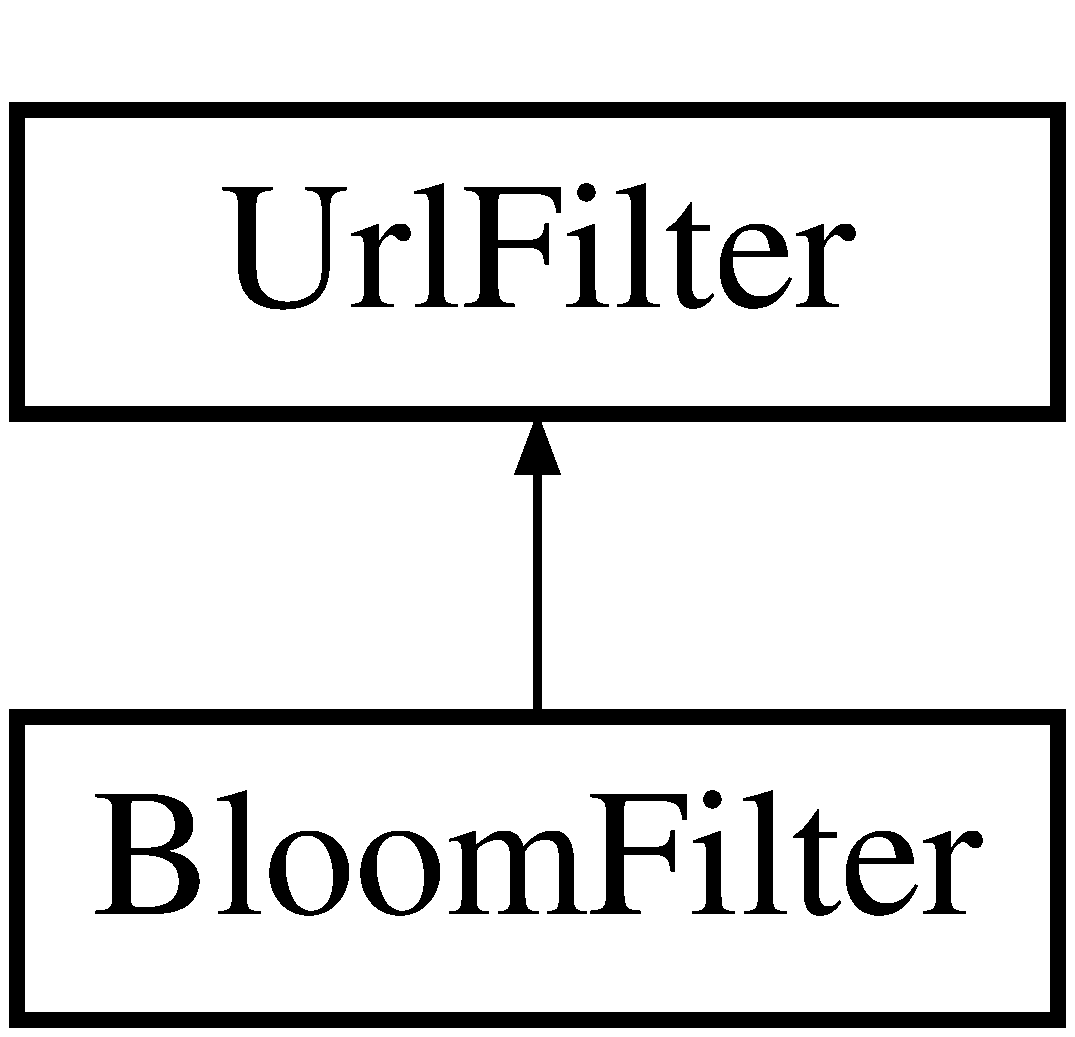
\includegraphics[height=2.000000cm]{class_bloom_filter}
\end{center}
\end{figure}
\subsection*{Public Member Functions}
\begin{DoxyCompactItemize}
\item 
\mbox{\Hypertarget{class_bloom_filter_a4e78efdfb6b1a240ab58d9f1cdea3c48}\label{class_bloom_filter_a4e78efdfb6b1a240ab58d9f1cdea3c48}} 
\hyperlink{class_bloom_filter_a4e78efdfb6b1a240ab58d9f1cdea3c48}{Bloom\+Filter} (void)
\begin{DoxyCompactList}\small\item\em 构造器 \end{DoxyCompactList}\item 
bool \hyperlink{class_bloom_filter_a78a992167b8efbc3be672469e68c5e97}{exist} (string const \&str\+Url)
\begin{DoxyCompactList}\small\item\em 判断某个统一资源定位符是否已经存在 \end{DoxyCompactList}\end{DoxyCompactItemize}


\subsection{Detailed Description}
布隆过滤器 

\subsection{Member Function Documentation}
\mbox{\Hypertarget{class_bloom_filter_a78a992167b8efbc3be672469e68c5e97}\label{class_bloom_filter_a78a992167b8efbc3be672469e68c5e97}} 
\index{Bloom\+Filter@{Bloom\+Filter}!exist@{exist}}
\index{exist@{exist}!Bloom\+Filter@{Bloom\+Filter}}
\subsubsection{\texorpdfstring{exist()}{exist()}}
{\footnotesize\ttfamily bool Bloom\+Filter\+::exist (\begin{DoxyParamCaption}\item[{string const \&}]{str\+Url }\end{DoxyParamCaption})\hspace{0.3cm}{\ttfamily [virtual]}}



判断某个统一资源定位符是否已经存在 


\begin{DoxyRetVals}{Return values}
{\em true} & 存在 \\
\hline
{\em false} & 不存在,同时将其加入布隆表 \\
\hline
\end{DoxyRetVals}
\begin{DoxyNote}{Note}
根据布隆过滤器的策略实现基类中的纯虚函数 
\end{DoxyNote}

\begin{DoxyParams}[1]{Parameters}
\mbox{\tt in}  & {\em str\+Url} & 统一资源定位符 \\
\hline
\end{DoxyParams}


Implements \hyperlink{class_url_filter_a581b9ea03daefbf52344ceb3371f409a}{Url\+Filter}.



The documentation for this class was generated from the following files\+:\begin{DoxyCompactItemize}
\item 
src/\hyperlink{_bloom_filter_8h}{Bloom\+Filter.\+h}\item 
src/\hyperlink{_bloom_filter_8cpp}{Bloom\+Filter.\+cpp}\end{DoxyCompactItemize}

\hypertarget{class_configurator}{}\section{Configurator Class Reference}
\label{class_configurator}\index{Configurator@{Configurator}}


配置器  




{\ttfamily \#include $<$Configurator.\+h$>$}

\subsection*{Public Member Functions}
\begin{DoxyCompactItemize}
\item 
\mbox{\Hypertarget{class_configurator_a8755c4fd8511b54067af1f1ac78ba18c}\label{class_configurator_a8755c4fd8511b54067af1f1ac78ba18c}} 
\hyperlink{class_configurator_a8755c4fd8511b54067af1f1ac78ba18c}{Configurator} (void)
\begin{DoxyCompactList}\small\item\em 构造器 \end{DoxyCompactList}\item 
void \hyperlink{class_configurator_a5c8b62b3619de64a81b3877a4498f6d8}{load} (string const \&cfg\+File)
\begin{DoxyCompactList}\small\item\em 从指定的配置文件中加载配置信息 \end{DoxyCompactList}\end{DoxyCompactItemize}
\subsection*{Public Attributes}
\begin{DoxyCompactItemize}
\item 
int \hyperlink{class_configurator_a48b66a5bd8038dd8a186c295111ed7ce}{m\+\_\+log\+Level}
\begin{DoxyCompactList}\small\item\em 最低日志等级 \end{DoxyCompactList}\item 
\mbox{\Hypertarget{class_configurator_adac0a4036fa93d7ea780e586befd5d32}\label{class_configurator_adac0a4036fa93d7ea780e586befd5d32}} 
string \hyperlink{class_configurator_adac0a4036fa93d7ea780e586befd5d32}{m\+\_\+log\+File}
\begin{DoxyCompactList}\small\item\em 日志文件路径 \end{DoxyCompactList}\item 
\mbox{\Hypertarget{class_configurator_a70acfa6e6928b1aab0ae7c9444b1a46e}\label{class_configurator_a70acfa6e6928b1aab0ae7c9444b1a46e}} 
int \hyperlink{class_configurator_a70acfa6e6928b1aab0ae7c9444b1a46e}{m\+\_\+max\+Jobs}
\begin{DoxyCompactList}\small\item\em 最大抓取任务数,0表示不抓取,-\/1表示无限抓取 \end{DoxyCompactList}\item 
\mbox{\Hypertarget{class_configurator_a20f4111bbd490936746422cb57cf72bd}\label{class_configurator_a20f4111bbd490936746422cb57cf72bd}} 
int \hyperlink{class_configurator_a20f4111bbd490936746422cb57cf72bd}{m\+\_\+max\+Depth}
\begin{DoxyCompactList}\small\item\em 最大递归深度,种子深度为0,之后逐层递增,-\/1表示无限深度 \end{DoxyCompactList}\item 
\mbox{\Hypertarget{class_configurator_a219d7b0dc18eb5b11fdbc5c0f83da32c}\label{class_configurator_a219d7b0dc18eb5b11fdbc5c0f83da32c}} 
int \hyperlink{class_configurator_a219d7b0dc18eb5b11fdbc5c0f83da32c}{m\+\_\+max\+Raw\+Urls}
\begin{DoxyCompactList}\small\item\em 原始统一资源定位符队列最大容量,-\/1表示无限大 \end{DoxyCompactList}\item 
\mbox{\Hypertarget{class_configurator_a3d64cd25dbfee1edf4d26fd642b629f3}\label{class_configurator_a3d64cd25dbfee1edf4d26fd642b629f3}} 
int \hyperlink{class_configurator_a3d64cd25dbfee1edf4d26fd642b629f3}{m\+\_\+max\+Dns\+Urls}
\begin{DoxyCompactList}\small\item\em 解析统一资源定位符队列最大容量,-\/1表示无限大 \end{DoxyCompactList}\item 
\mbox{\Hypertarget{class_configurator_abf473e476241dd69d7a0b3373f35f8dd}\label{class_configurator_abf473e476241dd69d7a0b3373f35f8dd}} 
long \hyperlink{class_configurator_abf473e476241dd69d7a0b3373f35f8dd}{m\+\_\+stat\+Interval}
\begin{DoxyCompactList}\small\item\em 状态间隔,即状态定时器的周期秒数,0表示不设定时器 \end{DoxyCompactList}\item 
\mbox{\Hypertarget{class_configurator_ac9c2b18d9fba05948495f793fdf66124}\label{class_configurator_ac9c2b18d9fba05948495f793fdf66124}} 
string \hyperlink{class_configurator_ac9c2b18d9fba05948495f793fdf66124}{m\+\_\+seeds}
\begin{DoxyCompactList}\small\item\em 种子链接,多个链接以逗号隔开 \end{DoxyCompactList}\item 
\mbox{\Hypertarget{class_configurator_a26310ca9cf9ee2757b6e5e145205d4b7}\label{class_configurator_a26310ca9cf9ee2757b6e5e145205d4b7}} 
string \hyperlink{class_configurator_a26310ca9cf9ee2757b6e5e145205d4b7}{m\+\_\+include\+Prefixes}
\begin{DoxyCompactList}\small\item\em 包含前缀,只抓取带有这些前缀的\+U\+R\+L,多个前缀以逗号隔开 \end{DoxyCompactList}\item 
\mbox{\Hypertarget{class_configurator_a4a88e7daaeffed59739ed8ec7619f3b7}\label{class_configurator_a4a88e7daaeffed59739ed8ec7619f3b7}} 
string \hyperlink{class_configurator_a4a88e7daaeffed59739ed8ec7619f3b7}{m\+\_\+exclude\+Prefixes}
\begin{DoxyCompactList}\small\item\em 排除前缀,不抓取带有这些前缀的\+U\+R\+L,多个前缀以逗号隔开 \end{DoxyCompactList}\item 
\mbox{\Hypertarget{class_configurator_ad85f230b1fb317a9067769d8ab64805d}\label{class_configurator_ad85f230b1fb317a9067769d8ab64805d}} 
string \hyperlink{class_configurator_ad85f230b1fb317a9067769d8ab64805d}{m\+\_\+plugins\+Path}
\begin{DoxyCompactList}\small\item\em 插件路径 \end{DoxyCompactList}\item 
\mbox{\Hypertarget{class_configurator_ade960dc8653e08ba447b18fa1561cbef}\label{class_configurator_ade960dc8653e08ba447b18fa1561cbef}} 
vector$<$ string $>$ \hyperlink{class_configurator_ade960dc8653e08ba447b18fa1561cbef}{m\+\_\+load\+Plugins}
\begin{DoxyCompactList}\small\item\em 插件列表 \end{DoxyCompactList}\item 
\mbox{\Hypertarget{class_configurator_a6683f77519f28b12e3296a4457da502b}\label{class_configurator_a6683f77519f28b12e3296a4457da502b}} 
vector$<$ string $>$ \hyperlink{class_configurator_a6683f77519f28b12e3296a4457da502b}{m\+\_\+accept\+Types}
\begin{DoxyCompactList}\small\item\em 接受类型 \end{DoxyCompactList}\end{DoxyCompactItemize}


\subsection{Detailed Description}
配置器 

\subsection{Member Function Documentation}
\mbox{\Hypertarget{class_configurator_a5c8b62b3619de64a81b3877a4498f6d8}\label{class_configurator_a5c8b62b3619de64a81b3877a4498f6d8}} 
\index{Configurator@{Configurator}!load@{load}}
\index{load@{load}!Configurator@{Configurator}}
\subsubsection{\texorpdfstring{load()}{load()}}
{\footnotesize\ttfamily void Configurator\+::load (\begin{DoxyParamCaption}\item[{string const \&}]{cfg\+File }\end{DoxyParamCaption})}



从指定的配置文件中加载配置信息 


\begin{DoxyParams}[1]{Parameters}
\mbox{\tt in}  & {\em cfg\+File} & 配置文件路径 \\
\hline
\end{DoxyParams}


\subsection{Member Data Documentation}
\mbox{\Hypertarget{class_configurator_a48b66a5bd8038dd8a186c295111ed7ce}\label{class_configurator_a48b66a5bd8038dd8a186c295111ed7ce}} 
\index{Configurator@{Configurator}!m\+\_\+log\+Level@{m\+\_\+log\+Level}}
\index{m\+\_\+log\+Level@{m\+\_\+log\+Level}!Configurator@{Configurator}}
\subsubsection{\texorpdfstring{m\+\_\+log\+Level}{m\_logLevel}}
{\footnotesize\ttfamily int Configurator\+::m\+\_\+log\+Level}



最低日志等级 

从低到高依次为:
\begin{DoxyItemize}
\item 0 -\/ 调试
\item 1 -\/ 信息
\item 2 -\/ 警告
\item 3 -\/ 错误
\item 4 -\/ 致命
\end{DoxyItemize}系统将记录所有不低于指定等级的日志信息 

The documentation for this class was generated from the following files\+:\begin{DoxyCompactItemize}
\item 
src/\hyperlink{_configurator_8h}{Configurator.\+h}\item 
src/\hyperlink{_configurator_8cpp}{Configurator.\+cpp}\end{DoxyCompactItemize}

\hypertarget{class_dns_thread}{}\section{Dns\+Thread Class Reference}
\label{class_dns_thread}\index{Dns\+Thread@{Dns\+Thread}}


域名解析线程  




{\ttfamily \#include $<$Dns\+Thread.\+h$>$}

Inheritance diagram for Dns\+Thread\+:\begin{figure}[H]
\begin{center}
\leavevmode
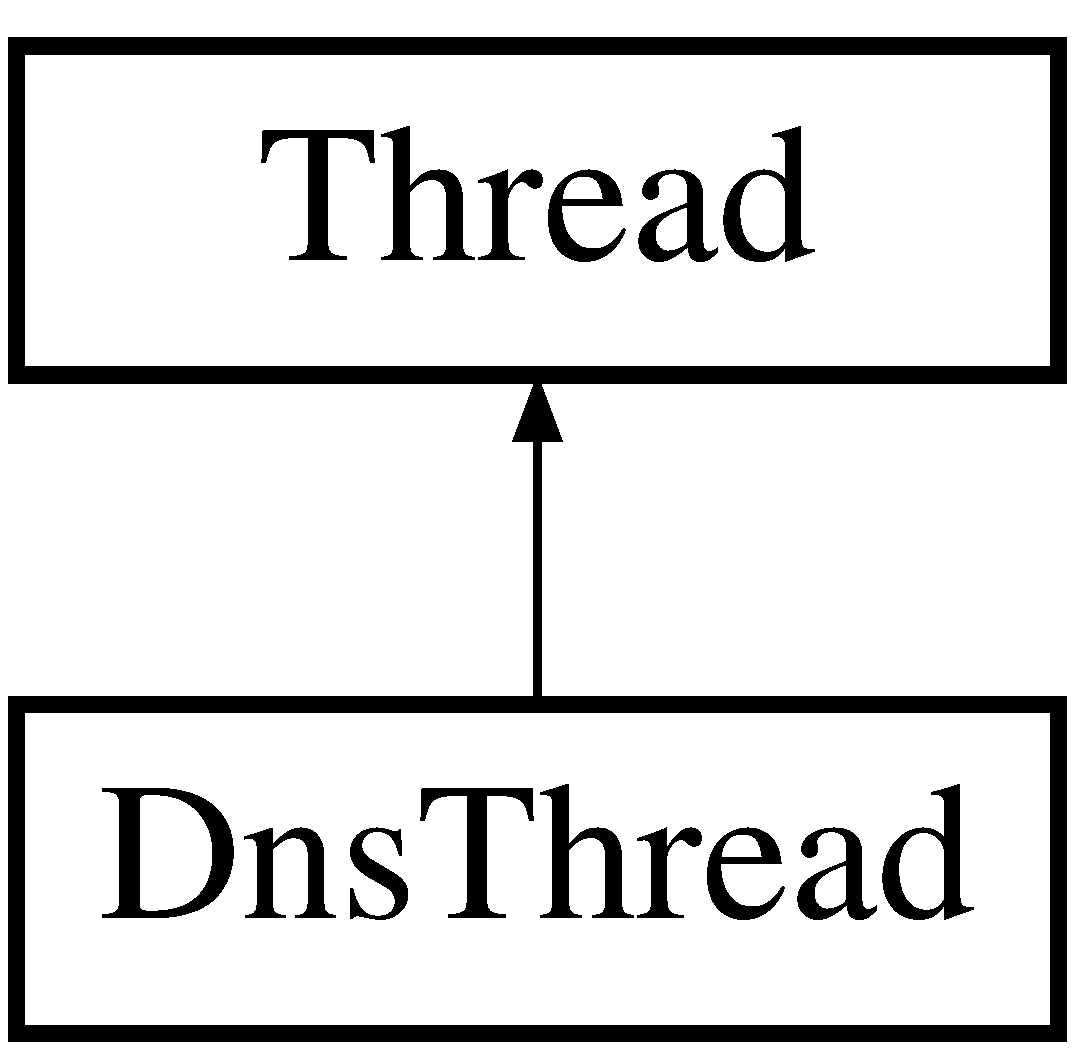
\includegraphics[height=2.000000cm]{class_dns_thread}
\end{center}
\end{figure}
\subsection*{Additional Inherited Members}


\subsection{Detailed Description}
域名解析线程 

The documentation for this class was generated from the following files\+:\begin{DoxyCompactItemize}
\item 
src/\hyperlink{_dns_thread_8h}{Dns\+Thread.\+h}\item 
src/\hyperlink{_dns_thread_8cpp}{Dns\+Thread.\+cpp}\end{DoxyCompactItemize}

\hypertarget{class_dns_url}{}\section{Dns\+Url Class Reference}
\label{class_dns_url}\index{Dns\+Url@{Dns\+Url}}


解析统一资源定位符  




{\ttfamily \#include $<$Url.\+h$>$}

Inheritance diagram for Dns\+Url\+:\begin{figure}[H]
\begin{center}
\leavevmode
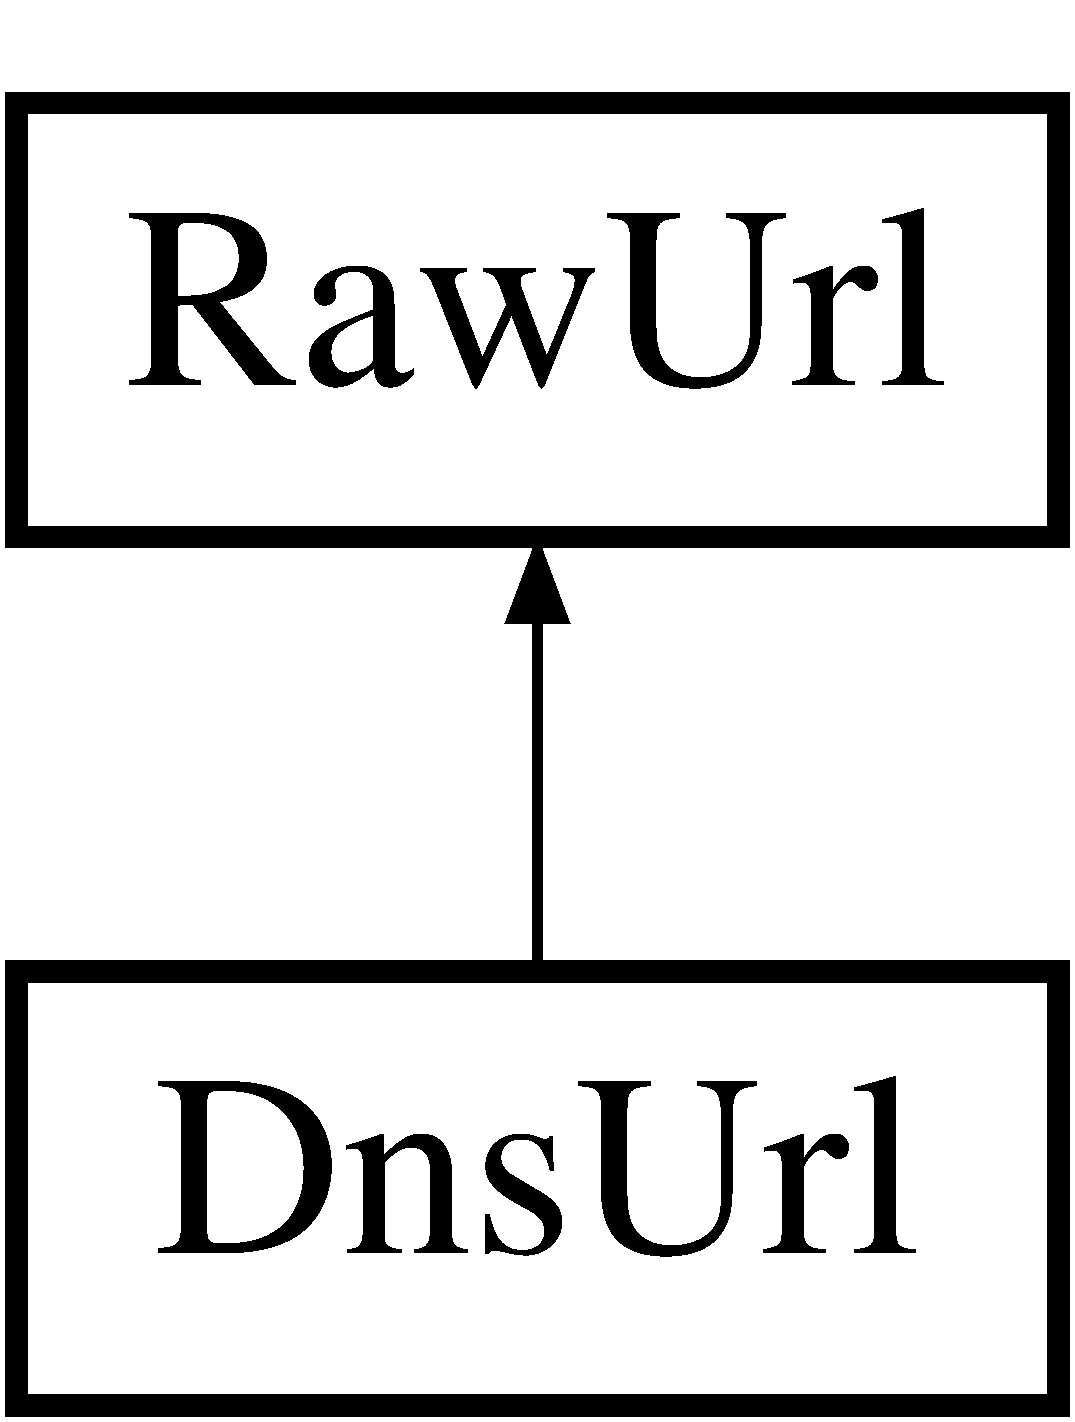
\includegraphics[height=2.000000cm]{class_dns_url}
\end{center}
\end{figure}
\subsection*{Public Member Functions}
\begin{DoxyCompactItemize}
\item 
\hyperlink{class_dns_url_a755c96cfb2eb70b9a39585553424f435}{Dns\+Url} (\hyperlink{class_raw_url}{Raw\+Url} const \&raw\+Url)
\begin{DoxyCompactList}\small\item\em 构造器 \end{DoxyCompactList}\item 
string \hyperlink{class_dns_url_a74cec9202ecf7631d02f53dcc498a4c6}{to\+Filename} (void) const
\begin{DoxyCompactList}\small\item\em 转换为文件名字符串 \end{DoxyCompactList}\item 
bool \hyperlink{class_dns_url_a96e4aa0b84d4bf4a693eed04ea7de4ca}{attach\+Domain} (string \&str\+Url) const
\begin{DoxyCompactList}\small\item\em 添加域名 \end{DoxyCompactList}\end{DoxyCompactItemize}
\subsection*{Public Attributes}
\begin{DoxyCompactItemize}
\item 
\mbox{\Hypertarget{class_dns_url_ad9f701802bbd22f6d6be49dc79a00eb5}\label{class_dns_url_ad9f701802bbd22f6d6be49dc79a00eb5}} 
string \hyperlink{class_dns_url_ad9f701802bbd22f6d6be49dc79a00eb5}{m\+\_\+domain}
\begin{DoxyCompactList}\small\item\em 服务器域名 \end{DoxyCompactList}\item 
\mbox{\Hypertarget{class_dns_url_ae7833d53958fbaab4de95d4406c5943d}\label{class_dns_url_ae7833d53958fbaab4de95d4406c5943d}} 
string \hyperlink{class_dns_url_ae7833d53958fbaab4de95d4406c5943d}{m\+\_\+path}
\begin{DoxyCompactList}\small\item\em 资源路径 \end{DoxyCompactList}\item 
\mbox{\Hypertarget{class_dns_url_a10a0576c9e2fb2a9179f27e10a3dc3ef}\label{class_dns_url_a10a0576c9e2fb2a9179f27e10a3dc3ef}} 
string \hyperlink{class_dns_url_a10a0576c9e2fb2a9179f27e10a3dc3ef}{m\+\_\+ip}
\begin{DoxyCompactList}\small\item\em 服务器\+I\+P地址 \end{DoxyCompactList}\item 
\mbox{\Hypertarget{class_dns_url_a471067dc236c12e337f7b25e771f2f74}\label{class_dns_url_a471067dc236c12e337f7b25e771f2f74}} 
short \hyperlink{class_dns_url_a471067dc236c12e337f7b25e771f2f74}{m\+\_\+port}
\begin{DoxyCompactList}\small\item\em 服务器通信端口 \end{DoxyCompactList}\end{DoxyCompactItemize}
\subsection*{Additional Inherited Members}


\subsection{Detailed Description}
解析统一资源定位符 

\subsection{Constructor \& Destructor Documentation}
\mbox{\Hypertarget{class_dns_url_a755c96cfb2eb70b9a39585553424f435}\label{class_dns_url_a755c96cfb2eb70b9a39585553424f435}} 
\index{Dns\+Url@{Dns\+Url}!Dns\+Url@{Dns\+Url}}
\index{Dns\+Url@{Dns\+Url}!Dns\+Url@{Dns\+Url}}
\subsubsection{\texorpdfstring{Dns\+Url()}{DnsUrl()}}
{\footnotesize\ttfamily Dns\+Url\+::\+Dns\+Url (\begin{DoxyParamCaption}\item[{\hyperlink{class_raw_url}{Raw\+Url} const \&}]{raw\+Url }\end{DoxyParamCaption})\hspace{0.3cm}{\ttfamily [explicit]}}



构造器 


\begin{DoxyParams}[1]{Parameters}
\mbox{\tt in}  & {\em raw\+Url} & 原始统一资源定位符 \\
\hline
\end{DoxyParams}


\subsection{Member Function Documentation}
\mbox{\Hypertarget{class_dns_url_a96e4aa0b84d4bf4a693eed04ea7de4ca}\label{class_dns_url_a96e4aa0b84d4bf4a693eed04ea7de4ca}} 
\index{Dns\+Url@{Dns\+Url}!attach\+Domain@{attach\+Domain}}
\index{attach\+Domain@{attach\+Domain}!Dns\+Url@{Dns\+Url}}
\subsubsection{\texorpdfstring{attach\+Domain()}{attachDomain()}}
{\footnotesize\ttfamily bool Dns\+Url\+::attach\+Domain (\begin{DoxyParamCaption}\item[{string \&}]{str\+Url }\end{DoxyParamCaption}) const}



添加域名 


\begin{DoxyRetVals}{Return values}
{\em true} & 成功 \\
\hline
{\em false} & 失败 \\
\hline
\end{DoxyRetVals}

\begin{DoxyParams}[1]{Parameters}
\mbox{\tt in,out}  & {\em str\+Url} & 待加域名统一资源定位符字符串 \\
\hline
\end{DoxyParams}
\mbox{\Hypertarget{class_dns_url_a74cec9202ecf7631d02f53dcc498a4c6}\label{class_dns_url_a74cec9202ecf7631d02f53dcc498a4c6}} 
\index{Dns\+Url@{Dns\+Url}!to\+Filename@{to\+Filename}}
\index{to\+Filename@{to\+Filename}!Dns\+Url@{Dns\+Url}}
\subsubsection{\texorpdfstring{to\+Filename()}{toFilename()}}
{\footnotesize\ttfamily string Dns\+Url\+::to\+Filename (\begin{DoxyParamCaption}\item[{void}]{ }\end{DoxyParamCaption}) const}



转换为文件名字符串 

\begin{DoxyReturn}{Returns}
文件名字符串 
\end{DoxyReturn}


The documentation for this class was generated from the following files\+:\begin{DoxyCompactItemize}
\item 
src/\hyperlink{_url_8h}{Url.\+h}\item 
src/\hyperlink{_url_8cpp}{Url.\+cpp}\end{DoxyCompactItemize}

\hypertarget{class_hash}{}\section{Hash Class Reference}
\label{class_hash}\index{Hash@{Hash}}


哈希器  




{\ttfamily \#include $<$Hash.\+h$>$}

\subsection*{Public Member Functions}
\begin{DoxyCompactItemize}
\item 
\mbox{\Hypertarget{class_hash_a73664aa35c78765aff5ef005db70d245}\label{class_hash_a73664aa35c78765aff5ef005db70d245}} 
\hyperlink{class_hash_a73664aa35c78765aff5ef005db70d245}{Hash} (void)
\begin{DoxyCompactList}\small\item\em 构造器 \end{DoxyCompactList}\item 
unsigned int \hyperlink{class_hash_a0600339cc7fef22914aab8e066f91fae}{times33} (string const \&str) const
\begin{DoxyCompactList}\small\item\em Times33哈希算法 \end{DoxyCompactList}\item 
unsigned int \hyperlink{class_hash_a67ee2152ea8e40b60b2c395c83cecc6f}{timesnum} (string const \&str, int num) const
\begin{DoxyCompactList}\small\item\em Times\+N哈希算法 \end{DoxyCompactList}\item 
unsigned int \hyperlink{class_hash_a05d68fb8603e00eb7b2bce77fd6539c5}{aphash} (string const \&str) const
\begin{DoxyCompactList}\small\item\em A\+P哈希算法 \end{DoxyCompactList}\item 
unsigned int \hyperlink{class_hash_a87064dbb105ec1193050067e1eb564f5}{hash16777619} (string const \&str) const
\begin{DoxyCompactList}\small\item\em F\+N\+V哈希算法 \end{DoxyCompactList}\item 
unsigned int \hyperlink{class_hash_a1a557f44997810270c6d753802a22743}{mysqlhash} (string const \&str) const
\begin{DoxyCompactList}\small\item\em My\+S\+Q\+L哈希算法 \end{DoxyCompactList}\item 
unsigned int \hyperlink{class_hash_afc6d940f27dc7f056cd41c171bd46b4c}{crc32} (string const \&str) const
\begin{DoxyCompactList}\small\item\em 循环冗余校验算法 \end{DoxyCompactList}\end{DoxyCompactItemize}


\subsection{Detailed Description}
哈希器 

\subsection{Member Function Documentation}
\mbox{\Hypertarget{class_hash_a05d68fb8603e00eb7b2bce77fd6539c5}\label{class_hash_a05d68fb8603e00eb7b2bce77fd6539c5}} 
\index{Hash@{Hash}!aphash@{aphash}}
\index{aphash@{aphash}!Hash@{Hash}}
\subsubsection{\texorpdfstring{aphash()}{aphash()}}
{\footnotesize\ttfamily unsigned int Hash\+::aphash (\begin{DoxyParamCaption}\item[{string const \&}]{str }\end{DoxyParamCaption}) const}



A\+P哈希算法 

\begin{DoxyReturn}{Returns}
参数字符串的32位哈希值 
\end{DoxyReturn}

\begin{DoxyParams}[1]{Parameters}
\mbox{\tt in}  & {\em str} & 被哈希字符串 \\
\hline
\end{DoxyParams}
\mbox{\Hypertarget{class_hash_afc6d940f27dc7f056cd41c171bd46b4c}\label{class_hash_afc6d940f27dc7f056cd41c171bd46b4c}} 
\index{Hash@{Hash}!crc32@{crc32}}
\index{crc32@{crc32}!Hash@{Hash}}
\subsubsection{\texorpdfstring{crc32()}{crc32()}}
{\footnotesize\ttfamily unsigned int Hash\+::crc32 (\begin{DoxyParamCaption}\item[{string const \&}]{str }\end{DoxyParamCaption}) const}



循环冗余校验算法 

\begin{DoxyReturn}{Returns}
参数字符串的循环冗余校验码 
\end{DoxyReturn}

\begin{DoxyParams}[1]{Parameters}
\mbox{\tt in}  & {\em str} & 被校验字符串 \\
\hline
\end{DoxyParams}
\mbox{\Hypertarget{class_hash_a87064dbb105ec1193050067e1eb564f5}\label{class_hash_a87064dbb105ec1193050067e1eb564f5}} 
\index{Hash@{Hash}!hash16777619@{hash16777619}}
\index{hash16777619@{hash16777619}!Hash@{Hash}}
\subsubsection{\texorpdfstring{hash16777619()}{hash16777619()}}
{\footnotesize\ttfamily unsigned int Hash\+::hash16777619 (\begin{DoxyParamCaption}\item[{string const \&}]{str }\end{DoxyParamCaption}) const}



F\+N\+V哈希算法 

\begin{DoxyReturn}{Returns}
参数字符串的32位哈希值 
\end{DoxyReturn}

\begin{DoxyParams}[1]{Parameters}
\mbox{\tt in}  & {\em str} & 被哈希字符串 \\
\hline
\end{DoxyParams}
\mbox{\Hypertarget{class_hash_a1a557f44997810270c6d753802a22743}\label{class_hash_a1a557f44997810270c6d753802a22743}} 
\index{Hash@{Hash}!mysqlhash@{mysqlhash}}
\index{mysqlhash@{mysqlhash}!Hash@{Hash}}
\subsubsection{\texorpdfstring{mysqlhash()}{mysqlhash()}}
{\footnotesize\ttfamily unsigned int Hash\+::mysqlhash (\begin{DoxyParamCaption}\item[{string const \&}]{str }\end{DoxyParamCaption}) const}



My\+S\+Q\+L哈希算法 

\begin{DoxyReturn}{Returns}
参数字符串的32位哈希值 
\end{DoxyReturn}

\begin{DoxyParams}[1]{Parameters}
\mbox{\tt in}  & {\em str} & 被哈希字符串 \\
\hline
\end{DoxyParams}
\mbox{\Hypertarget{class_hash_a0600339cc7fef22914aab8e066f91fae}\label{class_hash_a0600339cc7fef22914aab8e066f91fae}} 
\index{Hash@{Hash}!times33@{times33}}
\index{times33@{times33}!Hash@{Hash}}
\subsubsection{\texorpdfstring{times33()}{times33()}}
{\footnotesize\ttfamily unsigned int Hash\+::times33 (\begin{DoxyParamCaption}\item[{string const \&}]{str }\end{DoxyParamCaption}) const}



Times33哈希算法 

\begin{DoxyReturn}{Returns}
参数字符串的32位哈希值 
\end{DoxyReturn}
\begin{DoxyRemark}{Remarks}
hash(i) = hash(i-\/1)×33+str\mbox{[}i\mbox{]} (hash(-\/1) = 0) 
\end{DoxyRemark}

\begin{DoxyParams}[1]{Parameters}
\mbox{\tt in}  & {\em str} & 被哈希字符串 \\
\hline
\end{DoxyParams}
\mbox{\Hypertarget{class_hash_a67ee2152ea8e40b60b2c395c83cecc6f}\label{class_hash_a67ee2152ea8e40b60b2c395c83cecc6f}} 
\index{Hash@{Hash}!timesnum@{timesnum}}
\index{timesnum@{timesnum}!Hash@{Hash}}
\subsubsection{\texorpdfstring{timesnum()}{timesnum()}}
{\footnotesize\ttfamily unsigned int Hash\+::timesnum (\begin{DoxyParamCaption}\item[{string const \&}]{str,  }\item[{int}]{num }\end{DoxyParamCaption}) const}



Times\+N哈希算法 

\begin{DoxyReturn}{Returns}
参数字符串的32位哈希值 
\end{DoxyReturn}
\begin{DoxyRemark}{Remarks}
hash(i) = hash(i-\/1)×\+N+str\mbox{[}i\mbox{]} (hash(-\/1) = 0) 
\end{DoxyRemark}

\begin{DoxyParams}[1]{Parameters}
\mbox{\tt in}  & {\em str} & 被哈希字符串 \\
\hline
\mbox{\tt in}  & {\em num} & N \\
\hline
\end{DoxyParams}


The documentation for this class was generated from the following files\+:\begin{DoxyCompactItemize}
\item 
src/\hyperlink{_hash_8h}{Hash.\+h}\item 
src/\hyperlink{_hash_8cpp}{Hash.\+cpp}\end{DoxyCompactItemize}

\hypertarget{class_http_header}{}\section{Http\+Header Class Reference}
\label{class_http_header}\index{Http\+Header@{Http\+Header}}


超文本传输协议响应包头  




{\ttfamily \#include $<$Http.\+h$>$}

\subsection*{Public Attributes}
\begin{DoxyCompactItemize}
\item 
\mbox{\Hypertarget{class_http_header_af12a581280636bfd124fb0c9170ca509}\label{class_http_header_af12a581280636bfd124fb0c9170ca509}} 
int \hyperlink{class_http_header_af12a581280636bfd124fb0c9170ca509}{m\+\_\+status\+Code}
\begin{DoxyCompactList}\small\item\em 状态码 \end{DoxyCompactList}\item 
\mbox{\Hypertarget{class_http_header_a5a0a7a47c6053bb5f81873dbb5899f56}\label{class_http_header_a5a0a7a47c6053bb5f81873dbb5899f56}} 
string \hyperlink{class_http_header_a5a0a7a47c6053bb5f81873dbb5899f56}{m\+\_\+content\+Type}
\begin{DoxyCompactList}\small\item\em 内容类型 \end{DoxyCompactList}\end{DoxyCompactItemize}


\subsection{Detailed Description}
超文本传输协议响应包头 

The documentation for this class was generated from the following file\+:\begin{DoxyCompactItemize}
\item 
src/\hyperlink{_http_8h}{Http.\+h}\end{DoxyCompactItemize}

\hypertarget{class_http_response}{}\section{Http\+Response Class Reference}
\label{class_http_response}\index{Http\+Response@{Http\+Response}}


超文本传输协议响应  




{\ttfamily \#include $<$Http.\+h$>$}

\subsection*{Public Member Functions}
\begin{DoxyCompactItemize}
\item 
\hyperlink{class_http_response_a85d8b6b97c7ca4334e2d37ad4425a7c2}{Http\+Response} (\hyperlink{class_dns_url}{Dns\+Url} const \&dns\+Url)
\begin{DoxyCompactList}\small\item\em 构造器 \end{DoxyCompactList}\item 
\mbox{\Hypertarget{class_http_response_a9a03a4b1585dbff76f8712d686469b82}\label{class_http_response_a9a03a4b1585dbff76f8712d686469b82}} 
\hyperlink{class_http_response_a9a03a4b1585dbff76f8712d686469b82}{$\sim$\+Http\+Response} (void)
\begin{DoxyCompactList}\small\item\em 析构器 \end{DoxyCompactList}\end{DoxyCompactItemize}
\subsection*{Public Attributes}
\begin{DoxyCompactItemize}
\item 
\mbox{\Hypertarget{class_http_response_a956ae19ba3b1c86ac6c6c2a5a07b5372}\label{class_http_response_a956ae19ba3b1c86ac6c6c2a5a07b5372}} 
\hyperlink{class_dns_url}{Dns\+Url} \hyperlink{class_http_response_a956ae19ba3b1c86ac6c6c2a5a07b5372}{m\+\_\+dns\+Url}
\begin{DoxyCompactList}\small\item\em 服务器统一资源定位符 \end{DoxyCompactList}\item 
\mbox{\Hypertarget{class_http_response_a0ede873315f84c9af5cf94f3d3c9631f}\label{class_http_response_a0ede873315f84c9af5cf94f3d3c9631f}} 
\hyperlink{class_http_header}{Http\+Header} \hyperlink{class_http_response_a0ede873315f84c9af5cf94f3d3c9631f}{m\+\_\+header}
\begin{DoxyCompactList}\small\item\em 超文本传输协议响应包头 \end{DoxyCompactList}\item 
\mbox{\Hypertarget{class_http_response_a143e1bd466942aaa12a5b9b30c93bfab}\label{class_http_response_a143e1bd466942aaa12a5b9b30c93bfab}} 
char $\ast$ \hyperlink{class_http_response_a143e1bd466942aaa12a5b9b30c93bfab}{m\+\_\+body}
\begin{DoxyCompactList}\small\item\em 超文本传输协议响应包体指针 \end{DoxyCompactList}\item 
\mbox{\Hypertarget{class_http_response_af81c653a13929c449e99ee9c5e0cca3b}\label{class_http_response_af81c653a13929c449e99ee9c5e0cca3b}} 
size\+\_\+t \hyperlink{class_http_response_af81c653a13929c449e99ee9c5e0cca3b}{m\+\_\+len}
\begin{DoxyCompactList}\small\item\em 超文本传输协议响应包体长度 \end{DoxyCompactList}\end{DoxyCompactItemize}


\subsection{Detailed Description}
超文本传输协议响应 

\subsection{Constructor \& Destructor Documentation}
\mbox{\Hypertarget{class_http_response_a85d8b6b97c7ca4334e2d37ad4425a7c2}\label{class_http_response_a85d8b6b97c7ca4334e2d37ad4425a7c2}} 
\index{Http\+Response@{Http\+Response}!Http\+Response@{Http\+Response}}
\index{Http\+Response@{Http\+Response}!Http\+Response@{Http\+Response}}
\subsubsection{\texorpdfstring{Http\+Response()}{HttpResponse()}}
{\footnotesize\ttfamily Http\+Response\+::\+Http\+Response (\begin{DoxyParamCaption}\item[{\hyperlink{class_dns_url}{Dns\+Url} const \&}]{dns\+Url }\end{DoxyParamCaption})\hspace{0.3cm}{\ttfamily [inline]}}



构造器 


\begin{DoxyParams}[1]{Parameters}
\mbox{\tt in}  & {\em dns\+Url} & 服务器统一资源定位符 \\
\hline
\end{DoxyParams}


The documentation for this class was generated from the following file\+:\begin{DoxyCompactItemize}
\item 
src/\hyperlink{_http_8h}{Http.\+h}\end{DoxyCompactItemize}

\hypertarget{class_log}{}\section{Log Class Reference}
\label{class_log}\index{Log@{Log}}


日志  




{\ttfamily \#include $<$Log.\+h$>$}

\subsection*{Public Member Functions}
\begin{DoxyCompactItemize}
\item 
void \hyperlink{class_log_ab91d69d448051c3d127c0dac54b7869b}{printf} (int level, char const $\ast$file, int line, char const $\ast$format,...) const
\begin{DoxyCompactList}\small\item\em 按格式打印日志 \end{DoxyCompactList}\end{DoxyCompactItemize}
\subsection*{Static Public Attributes}
\begin{DoxyCompactItemize}
\item 
\mbox{\Hypertarget{class_log_aa17bb8ca4d2192d32661c3c7ca05a3f6}\label{class_log_aa17bb8ca4d2192d32661c3c7ca05a3f6}} 
static int const \hyperlink{class_log_aa17bb8ca4d2192d32661c3c7ca05a3f6}{L\+E\+V\+E\+L\+\_\+\+D\+BG} = 0
\begin{DoxyCompactList}\small\item\em 日志等级 -\/ 调试 \end{DoxyCompactList}\item 
\mbox{\Hypertarget{class_log_a858c5b18fa5ba2b3030c0e19396b1f29}\label{class_log_a858c5b18fa5ba2b3030c0e19396b1f29}} 
static int const \hyperlink{class_log_a858c5b18fa5ba2b3030c0e19396b1f29}{L\+E\+V\+E\+L\+\_\+\+I\+NF} = 1
\begin{DoxyCompactList}\small\item\em 日志等级 -\/ 信息 \end{DoxyCompactList}\item 
\mbox{\Hypertarget{class_log_a944495af10e73c8aabfa5b8ec5790c33}\label{class_log_a944495af10e73c8aabfa5b8ec5790c33}} 
static int const \hyperlink{class_log_a944495af10e73c8aabfa5b8ec5790c33}{L\+E\+V\+E\+L\+\_\+\+W\+AR} = 2
\begin{DoxyCompactList}\small\item\em 日志等级 -\/ 警告 \end{DoxyCompactList}\item 
\mbox{\Hypertarget{class_log_a0a37b6e34e4662db8a9c6797a83a7348}\label{class_log_a0a37b6e34e4662db8a9c6797a83a7348}} 
static int const \hyperlink{class_log_a0a37b6e34e4662db8a9c6797a83a7348}{L\+E\+V\+E\+L\+\_\+\+E\+RR} = 3
\begin{DoxyCompactList}\small\item\em 日志等级 -\/ 一般错误 \end{DoxyCompactList}\item 
\mbox{\Hypertarget{class_log_a4ec0940f19651e80e6852da6c7069916}\label{class_log_a4ec0940f19651e80e6852da6c7069916}} 
static int const \hyperlink{class_log_a4ec0940f19651e80e6852da6c7069916}{L\+E\+V\+E\+L\+\_\+\+C\+RT} = 4
\begin{DoxyCompactList}\small\item\em 日志等级 -\/ 致命错误 \end{DoxyCompactList}\end{DoxyCompactItemize}


\subsection{Detailed Description}
日志 

\subsection{Member Function Documentation}
\mbox{\Hypertarget{class_log_ab91d69d448051c3d127c0dac54b7869b}\label{class_log_ab91d69d448051c3d127c0dac54b7869b}} 
\index{Log@{Log}!printf@{printf}}
\index{printf@{printf}!Log@{Log}}
\subsubsection{\texorpdfstring{printf()}{printf()}}
{\footnotesize\ttfamily void Log\+::printf (\begin{DoxyParamCaption}\item[{int}]{level,  }\item[{char const $\ast$}]{file,  }\item[{int}]{line,  }\item[{char const $\ast$}]{format,  }\item[{}]{... }\end{DoxyParamCaption}) const}



按格式打印日志 


\begin{DoxyParams}[1]{Parameters}
\mbox{\tt in}  & {\em level} & 日志等级 \\
\hline
\mbox{\tt in}  & {\em file} & 源码文件 \\
\hline
\mbox{\tt in}  & {\em line} & 源码行号 \\
\hline
\mbox{\tt in}  & {\em format} & 格式化串 \\
\hline
\end{DoxyParams}


The documentation for this class was generated from the following files\+:\begin{DoxyCompactItemize}
\item 
src/\hyperlink{_log_8h}{Log.\+h}\item 
src/\hyperlink{_log_8cpp}{Log.\+cpp}\end{DoxyCompactItemize}

\hypertarget{class_multi_io}{}\section{Multi\+Io Class Reference}
\label{class_multi_io}\index{Multi\+Io@{Multi\+Io}}


多路输入输出  




{\ttfamily \#include $<$Multi\+Io.\+h$>$}

\subsection*{Public Member Functions}
\begin{DoxyCompactItemize}
\item 
\mbox{\Hypertarget{class_multi_io_a36b33c460c20e55f060cd7a5d45cf987}\label{class_multi_io_a36b33c460c20e55f060cd7a5d45cf987}} 
\hyperlink{class_multi_io_a36b33c460c20e55f060cd7a5d45cf987}{Multi\+Io} (void)
\begin{DoxyCompactList}\small\item\em 构造器 \end{DoxyCompactList}\item 
\mbox{\Hypertarget{class_multi_io_adb76f15666679c952f2f5ac8a46fe457}\label{class_multi_io_adb76f15666679c952f2f5ac8a46fe457}} 
\hyperlink{class_multi_io_adb76f15666679c952f2f5ac8a46fe457}{$\sim$\+Multi\+Io} (void)
\begin{DoxyCompactList}\small\item\em 析构器 \end{DoxyCompactList}\item 
bool \hyperlink{class_multi_io_abfbf48636d495e4d8031b111aa39b292}{add} (int fd, epoll\+\_\+event \&event) const
\begin{DoxyCompactList}\small\item\em 增加需要被关注的输入输出事件 \end{DoxyCompactList}\item 
bool \hyperlink{class_multi_io_a2d87b0b65a615623a53477fbef0eeced}{del} (int fd, epoll\+\_\+event \&event) const
\begin{DoxyCompactList}\small\item\em 删除需要被关注的输入输出事件 \end{DoxyCompactList}\item 
int \hyperlink{class_multi_io_af42ad1d3a228e514b0c1536ab5f276d2}{wait} (epoll\+\_\+event events\mbox{[}$\,$\mbox{]}, int max, int timeout) const
\begin{DoxyCompactList}\small\item\em 等待所关注输入输出事件的发生 \end{DoxyCompactList}\end{DoxyCompactItemize}


\subsection{Detailed Description}
多路输入输出 

\subsection{Member Function Documentation}
\mbox{\Hypertarget{class_multi_io_abfbf48636d495e4d8031b111aa39b292}\label{class_multi_io_abfbf48636d495e4d8031b111aa39b292}} 
\index{Multi\+Io@{Multi\+Io}!add@{add}}
\index{add@{add}!Multi\+Io@{Multi\+Io}}
\subsubsection{\texorpdfstring{add()}{add()}}
{\footnotesize\ttfamily bool Multi\+Io\+::add (\begin{DoxyParamCaption}\item[{int}]{fd,  }\item[{epoll\+\_\+event \&}]{event }\end{DoxyParamCaption}) const}



增加需要被关注的输入输出事件 


\begin{DoxyRetVals}{Return values}
{\em true} & 成功 \\
\hline
{\em false} & 失败 \\
\hline
\end{DoxyRetVals}

\begin{DoxyParams}[1]{Parameters}
\mbox{\tt in}  & {\em fd} & 发生输入输出事件的文件描述符 \\
\hline
\mbox{\tt in}  & {\em event} & 事件描述结构 \\
\hline
\end{DoxyParams}
\mbox{\Hypertarget{class_multi_io_a2d87b0b65a615623a53477fbef0eeced}\label{class_multi_io_a2d87b0b65a615623a53477fbef0eeced}} 
\index{Multi\+Io@{Multi\+Io}!del@{del}}
\index{del@{del}!Multi\+Io@{Multi\+Io}}
\subsubsection{\texorpdfstring{del()}{del()}}
{\footnotesize\ttfamily bool Multi\+Io\+::del (\begin{DoxyParamCaption}\item[{int}]{fd,  }\item[{epoll\+\_\+event \&}]{event }\end{DoxyParamCaption}) const}



删除需要被关注的输入输出事件 


\begin{DoxyRetVals}{Return values}
{\em true} & 成功 \\
\hline
{\em false} & 失败 \\
\hline
\end{DoxyRetVals}

\begin{DoxyParams}[1]{Parameters}
\mbox{\tt in}  & {\em fd} & 发生输入输出事件的文件描述符 \\
\hline
\mbox{\tt in}  & {\em event} & 事件描述结构 \\
\hline
\end{DoxyParams}
\mbox{\Hypertarget{class_multi_io_af42ad1d3a228e514b0c1536ab5f276d2}\label{class_multi_io_af42ad1d3a228e514b0c1536ab5f276d2}} 
\index{Multi\+Io@{Multi\+Io}!wait@{wait}}
\index{wait@{wait}!Multi\+Io@{Multi\+Io}}
\subsubsection{\texorpdfstring{wait()}{wait()}}
{\footnotesize\ttfamily int Multi\+Io\+::wait (\begin{DoxyParamCaption}\item[{epoll\+\_\+event}]{events\mbox{[}$\,$\mbox{]},  }\item[{int}]{max,  }\item[{int}]{timeout }\end{DoxyParamCaption}) const}



等待所关注输入输出事件的发生 


\begin{DoxyRetVals}{Return values}
{\em $>$0} & 处于就绪状态的文件描述符数 \\
\hline
{\em 0} & 超时 \\
\hline
{\em -\/1} & 失败 \\
\hline
\end{DoxyRetVals}

\begin{DoxyParams}[1]{Parameters}
\mbox{\tt out}  & {\em events} & 事件描述结构数组 \\
\hline
\mbox{\tt in}  & {\em max} & 事件描述结构数组容量 \\
\hline
\mbox{\tt in}  & {\em timeout} & 超时毫秒数,0立即超时,-\/1无限超时 \\
\hline
\end{DoxyParams}


The documentation for this class was generated from the following files\+:\begin{DoxyCompactItemize}
\item 
src/\hyperlink{_multi_io_8h}{Multi\+Io.\+h}\item 
src/\hyperlink{_multi_io_8cpp}{Multi\+Io.\+cpp}\end{DoxyCompactItemize}

\hypertarget{class_plugin}{}\section{Plugin Class Reference}
\label{class_plugin}\index{Plugin@{Plugin}}


插件接口  




{\ttfamily \#include $<$Plugin.\+h$>$}

\subsection*{Public Member Functions}
\begin{DoxyCompactItemize}
\item 
\mbox{\Hypertarget{class_plugin_a14edb40a1a126f4a30496bc5c1724b88}\label{class_plugin_a14edb40a1a126f4a30496bc5c1724b88}} 
virtual \hyperlink{class_plugin_a14edb40a1a126f4a30496bc5c1724b88}{$\sim$\+Plugin} (void)
\begin{DoxyCompactList}\small\item\em 析构器 \end{DoxyCompactList}\item 
virtual bool \hyperlink{class_plugin_a5473f4276b9992fdaecdd0bc6db60d37}{init} (\hyperlink{class_web_crawler}{Web\+Crawler} $\ast$app)=0
\begin{DoxyCompactList}\small\item\em 插件初始化 \end{DoxyCompactList}\item 
virtual bool \hyperlink{class_plugin_a12c99361b63a4b808b6bbe40d1a5de1d}{handler} (void $\ast$arg)=0
\begin{DoxyCompactList}\small\item\em 插件处理 \end{DoxyCompactList}\end{DoxyCompactItemize}


\subsection{Detailed Description}
插件接口 

\subsection{Member Function Documentation}
\mbox{\Hypertarget{class_plugin_a12c99361b63a4b808b6bbe40d1a5de1d}\label{class_plugin_a12c99361b63a4b808b6bbe40d1a5de1d}} 
\index{Plugin@{Plugin}!handler@{handler}}
\index{handler@{handler}!Plugin@{Plugin}}
\subsubsection{\texorpdfstring{handler()}{handler()}}
{\footnotesize\ttfamily virtual bool Plugin\+::handler (\begin{DoxyParamCaption}\item[{void $\ast$}]{arg }\end{DoxyParamCaption})\hspace{0.3cm}{\ttfamily [pure virtual]}}



插件处理 


\begin{DoxyRetVals}{Return values}
{\em true} & 成功 \\
\hline
{\em false} & 失败 \\
\hline
\end{DoxyRetVals}
\begin{DoxyNote}{Note}
纯虚函数,子类根据不同插件的具体功能给出具体实现 
\end{DoxyNote}

\begin{DoxyParams}[1]{Parameters}
\mbox{\tt in,out}  & {\em arg} & 插件参数 \\
\hline
\end{DoxyParams}
\mbox{\Hypertarget{class_plugin_a5473f4276b9992fdaecdd0bc6db60d37}\label{class_plugin_a5473f4276b9992fdaecdd0bc6db60d37}} 
\index{Plugin@{Plugin}!init@{init}}
\index{init@{init}!Plugin@{Plugin}}
\subsubsection{\texorpdfstring{init()}{init()}}
{\footnotesize\ttfamily virtual bool Plugin\+::init (\begin{DoxyParamCaption}\item[{\hyperlink{class_web_crawler}{Web\+Crawler} $\ast$}]{app }\end{DoxyParamCaption})\hspace{0.3cm}{\ttfamily [pure virtual]}}



插件初始化 


\begin{DoxyRetVals}{Return values}
{\em true} & 成功 \\
\hline
{\em false} & 失败 \\
\hline
\end{DoxyRetVals}
\begin{DoxyNote}{Note}
纯虚函数,子类根据不同的插件功能给出具体实现 
\end{DoxyNote}

\begin{DoxyParams}[1]{Parameters}
\mbox{\tt in,out}  & {\em app} & 应用程序对象 \\
\hline
\end{DoxyParams}


The documentation for this class was generated from the following file\+:\begin{DoxyCompactItemize}
\item 
src/\hyperlink{_plugin_8h}{Plugin.\+h}\end{DoxyCompactItemize}

\hypertarget{class_plugin_mngr}{}\section{Plugin\+Mngr Class Reference}
\label{class_plugin_mngr}\index{Plugin\+Mngr@{Plugin\+Mngr}}


插件管理器  




{\ttfamily \#include $<$Plugin\+Mngr.\+h$>$}

\subsection*{Public Member Functions}
\begin{DoxyCompactItemize}
\item 
\mbox{\Hypertarget{class_plugin_mngr_a8fb487bb33fc83355d285231a86e4bf2}\label{class_plugin_mngr_a8fb487bb33fc83355d285231a86e4bf2}} 
void \hyperlink{class_plugin_mngr_a8fb487bb33fc83355d285231a86e4bf2}{load} (void)
\begin{DoxyCompactList}\small\item\em 加载插件 \end{DoxyCompactList}\item 
void \hyperlink{class_plugin_mngr_a016ae68984aa3c04a32eaf29a334b5d5}{register\+Url\+Plugin} (\hyperlink{class_plugin}{Plugin} $\ast$plugin)
\begin{DoxyCompactList}\small\item\em 注册统一资源定位符插件 \end{DoxyCompactList}\item 
void \hyperlink{class_plugin_mngr_a4b1e91927684b2f976ca97fb441baeb7}{register\+Header\+Plugin} (\hyperlink{class_plugin}{Plugin} $\ast$plugin)
\begin{DoxyCompactList}\small\item\em 注册超文本传输协议响应包头插件 \end{DoxyCompactList}\item 
void \hyperlink{class_plugin_mngr_a27dbc387de2030fbdf6df8e61922a340}{register\+Html\+Plugin} (\hyperlink{class_plugin}{Plugin} $\ast$plugin)
\begin{DoxyCompactList}\small\item\em 注册超文本标记语言插件 \end{DoxyCompactList}\item 
bool \hyperlink{class_plugin_mngr_a28131538a70ca1ec9458d843efb0351c}{invoke\+Url\+Plugins} (void $\ast$arg) const
\begin{DoxyCompactList}\small\item\em 调用统一资源定位符插件处理函数 \end{DoxyCompactList}\item 
bool \hyperlink{class_plugin_mngr_ac3d8362f2197873631b3e4893e40dfcd}{invoke\+Header\+Plugins} (void $\ast$arg) const
\begin{DoxyCompactList}\small\item\em 调用超文本传输协议响应包头插件处理函数 \end{DoxyCompactList}\item 
void \hyperlink{class_plugin_mngr_ab1279ac48a5c4088b4caf61047d2574b}{invoke\+Html\+Plugins} (void $\ast$arg) const
\begin{DoxyCompactList}\small\item\em 调用超文本标记语言插件处理函数 \end{DoxyCompactList}\end{DoxyCompactItemize}


\subsection{Detailed Description}
插件管理器 

\subsection{Member Function Documentation}
\mbox{\Hypertarget{class_plugin_mngr_ac3d8362f2197873631b3e4893e40dfcd}\label{class_plugin_mngr_ac3d8362f2197873631b3e4893e40dfcd}} 
\index{Plugin\+Mngr@{Plugin\+Mngr}!invoke\+Header\+Plugins@{invoke\+Header\+Plugins}}
\index{invoke\+Header\+Plugins@{invoke\+Header\+Plugins}!Plugin\+Mngr@{Plugin\+Mngr}}
\subsubsection{\texorpdfstring{invoke\+Header\+Plugins()}{invokeHeaderPlugins()}}
{\footnotesize\ttfamily bool Plugin\+Mngr\+::invoke\+Header\+Plugins (\begin{DoxyParamCaption}\item[{void $\ast$}]{arg }\end{DoxyParamCaption}) const}



调用超文本传输协议响应包头插件处理函数 


\begin{DoxyRetVals}{Return values}
{\em true} & 成功 \\
\hline
{\em false} & 失败 \\
\hline
\end{DoxyRetVals}
\begin{DoxyRemark}{Remarks}
依次调用每个超文本传输协议响应包头插件处理函数,只要有一个失败即返回失败 
\end{DoxyRemark}

\begin{DoxyParams}[1]{Parameters}
\mbox{\tt in,out}  & {\em arg} & 插件参数 \\
\hline
\end{DoxyParams}
\mbox{\Hypertarget{class_plugin_mngr_ab1279ac48a5c4088b4caf61047d2574b}\label{class_plugin_mngr_ab1279ac48a5c4088b4caf61047d2574b}} 
\index{Plugin\+Mngr@{Plugin\+Mngr}!invoke\+Html\+Plugins@{invoke\+Html\+Plugins}}
\index{invoke\+Html\+Plugins@{invoke\+Html\+Plugins}!Plugin\+Mngr@{Plugin\+Mngr}}
\subsubsection{\texorpdfstring{invoke\+Html\+Plugins()}{invokeHtmlPlugins()}}
{\footnotesize\ttfamily void Plugin\+Mngr\+::invoke\+Html\+Plugins (\begin{DoxyParamCaption}\item[{void $\ast$}]{arg }\end{DoxyParamCaption}) const}



调用超文本标记语言插件处理函数 

\begin{DoxyRemark}{Remarks}
依次调用每个超文本标记语言插件处理函数,忽略其成功失败 
\end{DoxyRemark}

\begin{DoxyParams}[1]{Parameters}
\mbox{\tt in,out}  & {\em arg} & 插件参数 \\
\hline
\end{DoxyParams}
\mbox{\Hypertarget{class_plugin_mngr_a28131538a70ca1ec9458d843efb0351c}\label{class_plugin_mngr_a28131538a70ca1ec9458d843efb0351c}} 
\index{Plugin\+Mngr@{Plugin\+Mngr}!invoke\+Url\+Plugins@{invoke\+Url\+Plugins}}
\index{invoke\+Url\+Plugins@{invoke\+Url\+Plugins}!Plugin\+Mngr@{Plugin\+Mngr}}
\subsubsection{\texorpdfstring{invoke\+Url\+Plugins()}{invokeUrlPlugins()}}
{\footnotesize\ttfamily bool Plugin\+Mngr\+::invoke\+Url\+Plugins (\begin{DoxyParamCaption}\item[{void $\ast$}]{arg }\end{DoxyParamCaption}) const}



调用统一资源定位符插件处理函数 


\begin{DoxyRetVals}{Return values}
{\em true} & 成功 \\
\hline
{\em false} & 失败 \\
\hline
\end{DoxyRetVals}
\begin{DoxyRemark}{Remarks}
依次调用每个统一资源定位符插件处理函数,只要有一个失败即返回失败 
\end{DoxyRemark}

\begin{DoxyParams}[1]{Parameters}
\mbox{\tt in,out}  & {\em arg} & 插件参数 \\
\hline
\end{DoxyParams}
\mbox{\Hypertarget{class_plugin_mngr_a4b1e91927684b2f976ca97fb441baeb7}\label{class_plugin_mngr_a4b1e91927684b2f976ca97fb441baeb7}} 
\index{Plugin\+Mngr@{Plugin\+Mngr}!register\+Header\+Plugin@{register\+Header\+Plugin}}
\index{register\+Header\+Plugin@{register\+Header\+Plugin}!Plugin\+Mngr@{Plugin\+Mngr}}
\subsubsection{\texorpdfstring{register\+Header\+Plugin()}{registerHeaderPlugin()}}
{\footnotesize\ttfamily void Plugin\+Mngr\+::register\+Header\+Plugin (\begin{DoxyParamCaption}\item[{\hyperlink{class_plugin}{Plugin} $\ast$}]{plugin }\end{DoxyParamCaption})}



注册超文本传输协议响应包头插件 

\begin{DoxyRemark}{Remarks}
超文本传输协议响应包头插件通过此接口将其自身注册到插件管理器中 
\end{DoxyRemark}

\begin{DoxyParams}[1]{Parameters}
\mbox{\tt in}  & {\em plugin} & 超文本传输协议响应包头插件 \\
\hline
\end{DoxyParams}
\mbox{\Hypertarget{class_plugin_mngr_a27dbc387de2030fbdf6df8e61922a340}\label{class_plugin_mngr_a27dbc387de2030fbdf6df8e61922a340}} 
\index{Plugin\+Mngr@{Plugin\+Mngr}!register\+Html\+Plugin@{register\+Html\+Plugin}}
\index{register\+Html\+Plugin@{register\+Html\+Plugin}!Plugin\+Mngr@{Plugin\+Mngr}}
\subsubsection{\texorpdfstring{register\+Html\+Plugin()}{registerHtmlPlugin()}}
{\footnotesize\ttfamily void Plugin\+Mngr\+::register\+Html\+Plugin (\begin{DoxyParamCaption}\item[{\hyperlink{class_plugin}{Plugin} $\ast$}]{plugin }\end{DoxyParamCaption})}



注册超文本标记语言插件 

\begin{DoxyRemark}{Remarks}
超文本标记语言插件通过此接口将其自身注册到插件管理器中 
\end{DoxyRemark}

\begin{DoxyParams}[1]{Parameters}
\mbox{\tt in}  & {\em plugin} & 超文本标记语言插件 \\
\hline
\end{DoxyParams}
\mbox{\Hypertarget{class_plugin_mngr_a016ae68984aa3c04a32eaf29a334b5d5}\label{class_plugin_mngr_a016ae68984aa3c04a32eaf29a334b5d5}} 
\index{Plugin\+Mngr@{Plugin\+Mngr}!register\+Url\+Plugin@{register\+Url\+Plugin}}
\index{register\+Url\+Plugin@{register\+Url\+Plugin}!Plugin\+Mngr@{Plugin\+Mngr}}
\subsubsection{\texorpdfstring{register\+Url\+Plugin()}{registerUrlPlugin()}}
{\footnotesize\ttfamily void Plugin\+Mngr\+::register\+Url\+Plugin (\begin{DoxyParamCaption}\item[{\hyperlink{class_plugin}{Plugin} $\ast$}]{plugin }\end{DoxyParamCaption})}



注册统一资源定位符插件 

\begin{DoxyRemark}{Remarks}
统一资源定位符插件通过此接口将其自身注册到插件管理器中 
\end{DoxyRemark}

\begin{DoxyParams}[1]{Parameters}
\mbox{\tt in}  & {\em plugin} & 统一资源定位符插件 \\
\hline
\end{DoxyParams}


The documentation for this class was generated from the following files\+:\begin{DoxyCompactItemize}
\item 
src/\hyperlink{_plugin_mngr_8h}{Plugin\+Mngr.\+h}\item 
src/\hyperlink{_plugin_mngr_8cpp}{Plugin\+Mngr.\+cpp}\end{DoxyCompactItemize}

\hypertarget{class_raw_url}{}\section{Raw\+Url Class Reference}
\label{class_raw_url}\index{Raw\+Url@{Raw\+Url}}


原始统一资源定位符  




{\ttfamily \#include $<$Url.\+h$>$}

Inheritance diagram for Raw\+Url\+:\begin{figure}[H]
\begin{center}
\leavevmode
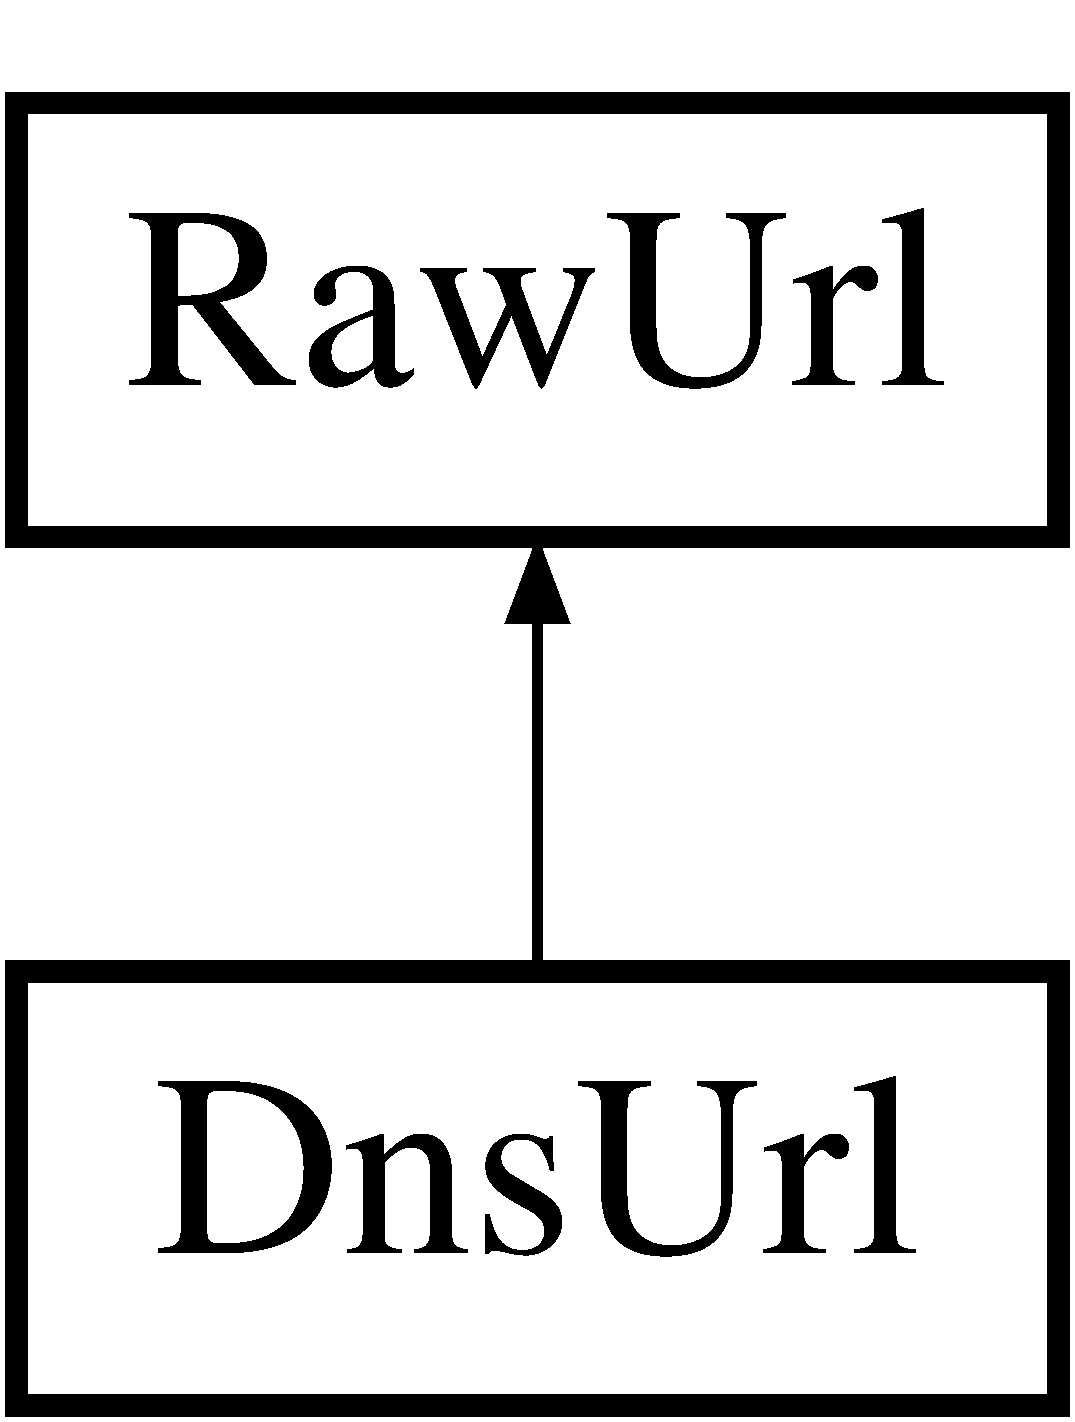
\includegraphics[height=2.000000cm]{class_raw_url}
\end{center}
\end{figure}
\subsection*{Public Types}
\begin{DoxyCompactItemize}
\item 
enum \hyperlink{class_raw_url_a193b4d2277a698b58643d1565cac278a}{tag\+\_\+\+Type} \{ \hyperlink{class_raw_url_a193b4d2277a698b58643d1565cac278aa6959b742b81c5a298a8a587f2ce5b955}{E\+T\+Y\+P\+E\+\_\+\+H\+T\+ML}, 
\hyperlink{class_raw_url_a193b4d2277a698b58643d1565cac278aa86232672f7dc4b0635d0716032a82390}{E\+T\+Y\+P\+E\+\_\+\+I\+M\+A\+GE}
 \}\begin{DoxyCompactList}\small\item\em 资源类型 \end{DoxyCompactList}
\item 
\mbox{\Hypertarget{class_raw_url_a6d7469b7f73d43e86e68d8c4182a7a51}\label{class_raw_url_a6d7469b7f73d43e86e68d8c4182a7a51}} 
typedef enum \hyperlink{class_raw_url_a193b4d2277a698b58643d1565cac278a}{Raw\+Url\+::tag\+\_\+\+Type} \hyperlink{class_raw_url_a6d7469b7f73d43e86e68d8c4182a7a51}{E\+T\+Y\+PE}
\begin{DoxyCompactList}\small\item\em 资源类型 \end{DoxyCompactList}\end{DoxyCompactItemize}
\subsection*{Public Member Functions}
\begin{DoxyCompactItemize}
\item 
\hyperlink{class_raw_url_a2f295fd2c4e3614531e38968c633433f}{Raw\+Url} (string const \&str\+Url, \hyperlink{class_raw_url_a6d7469b7f73d43e86e68d8c4182a7a51}{E\+T\+Y\+PE} type=\hyperlink{class_raw_url_a193b4d2277a698b58643d1565cac278aa6959b742b81c5a298a8a587f2ce5b955}{E\+T\+Y\+P\+E\+\_\+\+H\+T\+ML}, int depth=0)
\begin{DoxyCompactList}\small\item\em 构造器 \end{DoxyCompactList}\end{DoxyCompactItemize}
\subsection*{Static Public Member Functions}
\begin{DoxyCompactItemize}
\item 
static bool \hyperlink{class_raw_url_a12963416c125786ab585feed5a06fb19}{normalized} (string \&str\+Url)
\begin{DoxyCompactList}\small\item\em 规格化 \end{DoxyCompactList}\end{DoxyCompactItemize}
\subsection*{Public Attributes}
\begin{DoxyCompactItemize}
\item 
\mbox{\Hypertarget{class_raw_url_a58c17cc7793b26cd672fa95cf1cad1b7}\label{class_raw_url_a58c17cc7793b26cd672fa95cf1cad1b7}} 
string \hyperlink{class_raw_url_a58c17cc7793b26cd672fa95cf1cad1b7}{m\+\_\+str\+Url}
\begin{DoxyCompactList}\small\item\em 统一资源定位符字符串 \end{DoxyCompactList}\item 
\mbox{\Hypertarget{class_raw_url_aa4e0c2141471709af7b27af11b7d9568}\label{class_raw_url_aa4e0c2141471709af7b27af11b7d9568}} 
\hyperlink{class_raw_url_a6d7469b7f73d43e86e68d8c4182a7a51}{E\+T\+Y\+PE} \hyperlink{class_raw_url_aa4e0c2141471709af7b27af11b7d9568}{m\+\_\+type}
\begin{DoxyCompactList}\small\item\em 资源类型 \end{DoxyCompactList}\item 
\mbox{\Hypertarget{class_raw_url_aedd7e8ab35d070011a140d7466e2d25b}\label{class_raw_url_aedd7e8ab35d070011a140d7466e2d25b}} 
int \hyperlink{class_raw_url_aedd7e8ab35d070011a140d7466e2d25b}{m\+\_\+depth}
\begin{DoxyCompactList}\small\item\em 链接深度 \end{DoxyCompactList}\end{DoxyCompactItemize}


\subsection{Detailed Description}
原始统一资源定位符 

\subsection{Member Enumeration Documentation}
\mbox{\Hypertarget{class_raw_url_a193b4d2277a698b58643d1565cac278a}\label{class_raw_url_a193b4d2277a698b58643d1565cac278a}} 
\index{Raw\+Url@{Raw\+Url}!tag\+\_\+\+Type@{tag\+\_\+\+Type}}
\index{tag\+\_\+\+Type@{tag\+\_\+\+Type}!Raw\+Url@{Raw\+Url}}
\subsubsection{\texorpdfstring{tag\+\_\+\+Type}{tag\_Type}}
{\footnotesize\ttfamily enum \hyperlink{class_raw_url_a193b4d2277a698b58643d1565cac278a}{Raw\+Url\+::tag\+\_\+\+Type}}



资源类型 

\begin{DoxyEnumFields}{Enumerator}
\raisebox{\heightof{T}}[0pt][0pt]{\index{E\+T\+Y\+P\+E\+\_\+\+H\+T\+ML@{E\+T\+Y\+P\+E\+\_\+\+H\+T\+ML}!Raw\+Url@{Raw\+Url}}\index{Raw\+Url@{Raw\+Url}!E\+T\+Y\+P\+E\+\_\+\+H\+T\+ML@{E\+T\+Y\+P\+E\+\_\+\+H\+T\+ML}}}\mbox{\Hypertarget{class_raw_url_a193b4d2277a698b58643d1565cac278aa6959b742b81c5a298a8a587f2ce5b955}\label{class_raw_url_a193b4d2277a698b58643d1565cac278aa6959b742b81c5a298a8a587f2ce5b955}} 
E\+T\+Y\+P\+E\+\_\+\+H\+T\+ML&超文本标记语言 \\
\hline

\raisebox{\heightof{T}}[0pt][0pt]{\index{E\+T\+Y\+P\+E\+\_\+\+I\+M\+A\+GE@{E\+T\+Y\+P\+E\+\_\+\+I\+M\+A\+GE}!Raw\+Url@{Raw\+Url}}\index{Raw\+Url@{Raw\+Url}!E\+T\+Y\+P\+E\+\_\+\+I\+M\+A\+GE@{E\+T\+Y\+P\+E\+\_\+\+I\+M\+A\+GE}}}\mbox{\Hypertarget{class_raw_url_a193b4d2277a698b58643d1565cac278aa86232672f7dc4b0635d0716032a82390}\label{class_raw_url_a193b4d2277a698b58643d1565cac278aa86232672f7dc4b0635d0716032a82390}} 
E\+T\+Y\+P\+E\+\_\+\+I\+M\+A\+GE&图像 \\
\hline

\end{DoxyEnumFields}


\subsection{Constructor \& Destructor Documentation}
\mbox{\Hypertarget{class_raw_url_a2f295fd2c4e3614531e38968c633433f}\label{class_raw_url_a2f295fd2c4e3614531e38968c633433f}} 
\index{Raw\+Url@{Raw\+Url}!Raw\+Url@{Raw\+Url}}
\index{Raw\+Url@{Raw\+Url}!Raw\+Url@{Raw\+Url}}
\subsubsection{\texorpdfstring{Raw\+Url()}{RawUrl()}}
{\footnotesize\ttfamily Raw\+Url\+::\+Raw\+Url (\begin{DoxyParamCaption}\item[{string const \&}]{str\+Url,  }\item[{\hyperlink{class_raw_url_a6d7469b7f73d43e86e68d8c4182a7a51}{E\+T\+Y\+PE}}]{type = {\ttfamily \hyperlink{class_raw_url_a193b4d2277a698b58643d1565cac278aa6959b742b81c5a298a8a587f2ce5b955}{E\+T\+Y\+P\+E\+\_\+\+H\+T\+ML}},  }\item[{int}]{depth = {\ttfamily 0} }\end{DoxyParamCaption})}



构造器 


\begin{DoxyParams}[1]{Parameters}
\mbox{\tt in}  & {\em str\+Url} & 统一资源定位符字符串 \\
\hline
\mbox{\tt in}  & {\em type} & 资源类型 \\
\hline
\mbox{\tt in}  & {\em depth} & 链接深度 \\
\hline
\end{DoxyParams}


\subsection{Member Function Documentation}
\mbox{\Hypertarget{class_raw_url_a12963416c125786ab585feed5a06fb19}\label{class_raw_url_a12963416c125786ab585feed5a06fb19}} 
\index{Raw\+Url@{Raw\+Url}!normalized@{normalized}}
\index{normalized@{normalized}!Raw\+Url@{Raw\+Url}}
\subsubsection{\texorpdfstring{normalized()}{normalized()}}
{\footnotesize\ttfamily bool Raw\+Url\+::normalized (\begin{DoxyParamCaption}\item[{string \&}]{str\+Url }\end{DoxyParamCaption})\hspace{0.3cm}{\ttfamily [static]}}



规格化 


\begin{DoxyRetVals}{Return values}
{\em true} & 成功 \\
\hline
{\em false} & 失败 \\
\hline
\end{DoxyRetVals}
\begin{DoxyRemark}{Remarks}
删除协议标签(\href{http://}{\tt http\+://}或https\+://)和结尾分隔符(/) 
\end{DoxyRemark}

\begin{DoxyParams}[1]{Parameters}
\mbox{\tt in,out}  & {\em str\+Url} & 待规格化统一资源定位符字符串 \\
\hline
\end{DoxyParams}


The documentation for this class was generated from the following files\+:\begin{DoxyCompactItemize}
\item 
src/\hyperlink{_url_8h}{Url.\+h}\item 
src/\hyperlink{_url_8cpp}{Url.\+cpp}\end{DoxyCompactItemize}

\hypertarget{class_recv_thread}{}\section{Recv\+Thread Class Reference}
\label{class_recv_thread}\index{Recv\+Thread@{Recv\+Thread}}


接收线程  




{\ttfamily \#include $<$Recv\+Thread.\+h$>$}

Inheritance diagram for Recv\+Thread\+:\begin{figure}[H]
\begin{center}
\leavevmode
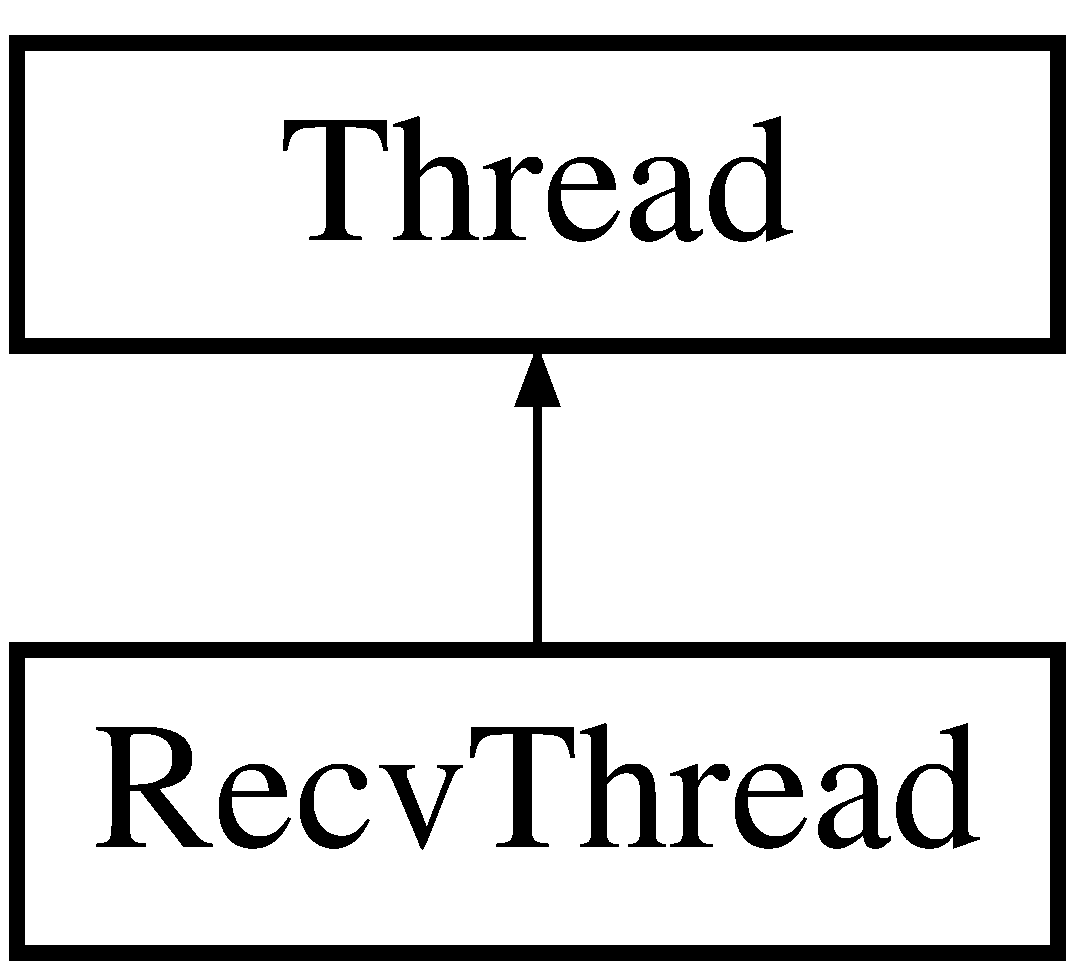
\includegraphics[height=2.000000cm]{class_recv_thread}
\end{center}
\end{figure}
\subsection*{Public Member Functions}
\begin{DoxyCompactItemize}
\item 
\hyperlink{class_recv_thread_af0ac3e83c4b9a049d9acdeabbbf6721a}{Recv\+Thread} (\hyperlink{class_socket}{Socket} $\ast$socket)
\begin{DoxyCompactList}\small\item\em 构造器 \end{DoxyCompactList}\item 
\mbox{\Hypertarget{class_recv_thread_a82c00d01fe10af0b6fd6a8d55fc168be}\label{class_recv_thread_a82c00d01fe10af0b6fd6a8d55fc168be}} 
\hyperlink{class_recv_thread_a82c00d01fe10af0b6fd6a8d55fc168be}{$\sim$\+Recv\+Thread} (void)
\begin{DoxyCompactList}\small\item\em 析构器 \end{DoxyCompactList}\end{DoxyCompactItemize}


\subsection{Detailed Description}
接收线程 

\subsection{Constructor \& Destructor Documentation}
\mbox{\Hypertarget{class_recv_thread_af0ac3e83c4b9a049d9acdeabbbf6721a}\label{class_recv_thread_af0ac3e83c4b9a049d9acdeabbbf6721a}} 
\index{Recv\+Thread@{Recv\+Thread}!Recv\+Thread@{Recv\+Thread}}
\index{Recv\+Thread@{Recv\+Thread}!Recv\+Thread@{Recv\+Thread}}
\subsubsection{\texorpdfstring{Recv\+Thread()}{RecvThread()}}
{\footnotesize\ttfamily Recv\+Thread\+::\+Recv\+Thread (\begin{DoxyParamCaption}\item[{\hyperlink{class_socket}{Socket} $\ast$}]{socket }\end{DoxyParamCaption})}



构造器 


\begin{DoxyParams}[1]{Parameters}
\mbox{\tt in}  & {\em socket} & 套接字 \\
\hline
\end{DoxyParams}


The documentation for this class was generated from the following files\+:\begin{DoxyCompactItemize}
\item 
src/\hyperlink{_recv_thread_8h}{Recv\+Thread.\+h}\item 
src/\hyperlink{_recv_thread_8cpp}{Recv\+Thread.\+cpp}\end{DoxyCompactItemize}

\hypertarget{class_send_thread}{}\section{Send\+Thread Class Reference}
\label{class_send_thread}\index{Send\+Thread@{Send\+Thread}}


发送线程  




{\ttfamily \#include $<$Send\+Thread.\+h$>$}

Inheritance diagram for Send\+Thread\+:\begin{figure}[H]
\begin{center}
\leavevmode
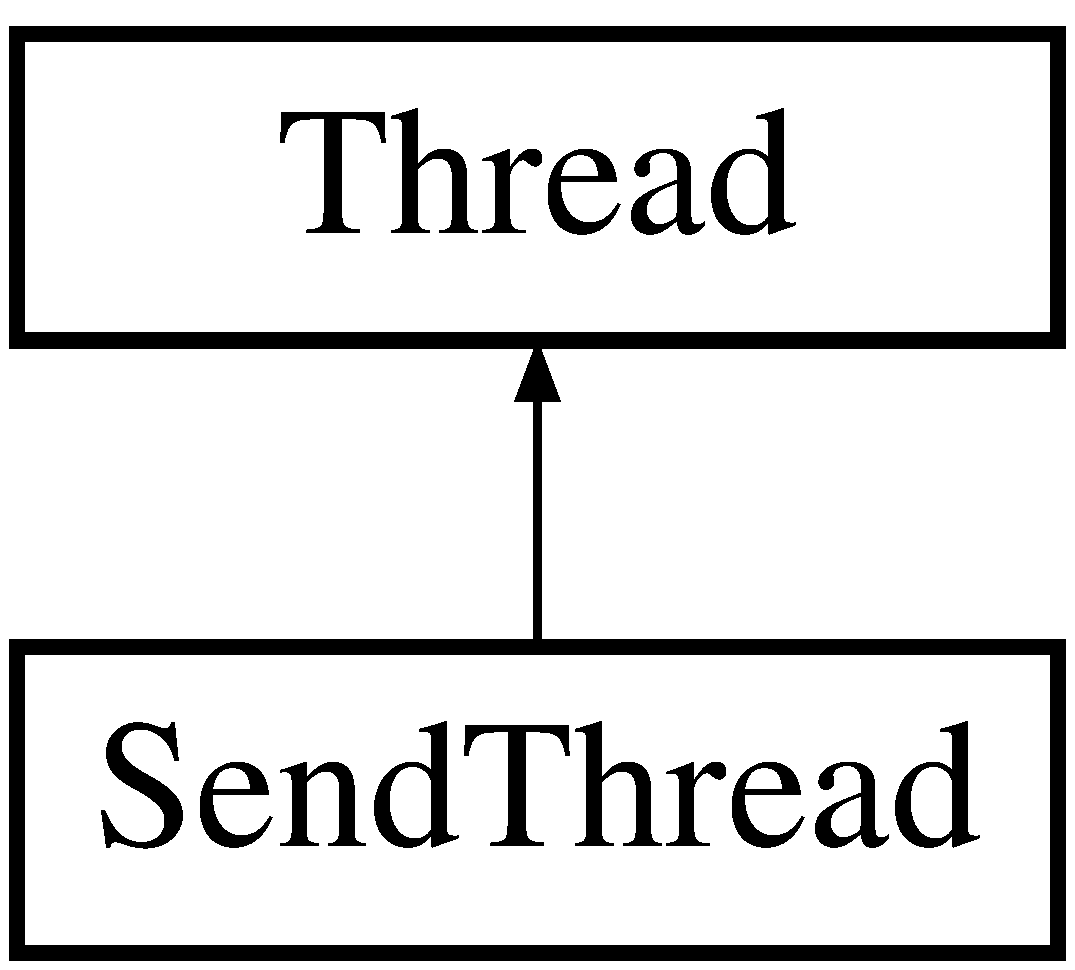
\includegraphics[height=2.000000cm]{class_send_thread}
\end{center}
\end{figure}
\subsection*{Additional Inherited Members}


\subsection{Detailed Description}
发送线程 

The documentation for this class was generated from the following files\+:\begin{DoxyCompactItemize}
\item 
src/\hyperlink{_send_thread_8h}{Send\+Thread.\+h}\item 
src/\hyperlink{_send_thread_8cpp}{Send\+Thread.\+cpp}\end{DoxyCompactItemize}

\hypertarget{class_socket}{}\section{Socket Class Reference}
\label{class_socket}\index{Socket@{Socket}}


套接字  




{\ttfamily \#include $<$Socket.\+h$>$}

\subsection*{Public Member Functions}
\begin{DoxyCompactItemize}
\item 
\hyperlink{class_socket_a57f6077d6f5db44a5eb8624463ed99e4}{Socket} (\hyperlink{class_dns_url}{Dns\+Url} const \&dns\+Url)
\begin{DoxyCompactList}\small\item\em 构造器 \end{DoxyCompactList}\item 
\mbox{\Hypertarget{class_socket_a763aae809efa471def8e7918281c3a1c}\label{class_socket_a763aae809efa471def8e7918281c3a1c}} 
\hyperlink{class_socket_a763aae809efa471def8e7918281c3a1c}{$\sim$\+Socket} (void)
\begin{DoxyCompactList}\small\item\em 析构器 \end{DoxyCompactList}\item 
bool \hyperlink{class_socket_acfc00252e4e40f68442a4b28fc5b32b3}{send\+Request} (void)
\begin{DoxyCompactList}\small\item\em 发送超文本传输协议请求 \end{DoxyCompactList}\item 
bool \hyperlink{class_socket_aa935a43a54d0ac03505b2ab32c095b99}{recv\+Response} (void)
\begin{DoxyCompactList}\small\item\em 接收超文本传输协议响应 \end{DoxyCompactList}\item 
int \hyperlink{class_socket_a427f1295ef1fce2c69e0b9a093fd0284}{sockfd} (void) const
\begin{DoxyCompactList}\small\item\em 获取套接字描述符 \end{DoxyCompactList}\end{DoxyCompactItemize}


\subsection{Detailed Description}
套接字 

\subsection{Constructor \& Destructor Documentation}
\mbox{\Hypertarget{class_socket_a57f6077d6f5db44a5eb8624463ed99e4}\label{class_socket_a57f6077d6f5db44a5eb8624463ed99e4}} 
\index{Socket@{Socket}!Socket@{Socket}}
\index{Socket@{Socket}!Socket@{Socket}}
\subsubsection{\texorpdfstring{Socket()}{Socket()}}
{\footnotesize\ttfamily Socket\+::\+Socket (\begin{DoxyParamCaption}\item[{\hyperlink{class_dns_url}{Dns\+Url} const \&}]{dns\+Url }\end{DoxyParamCaption})}



构造器 


\begin{DoxyParams}[1]{Parameters}
\mbox{\tt in}  & {\em dns\+Url} & 服务器统一资源定位符 \\
\hline
\end{DoxyParams}


\subsection{Member Function Documentation}
\mbox{\Hypertarget{class_socket_aa935a43a54d0ac03505b2ab32c095b99}\label{class_socket_aa935a43a54d0ac03505b2ab32c095b99}} 
\index{Socket@{Socket}!recv\+Response@{recv\+Response}}
\index{recv\+Response@{recv\+Response}!Socket@{Socket}}
\subsubsection{\texorpdfstring{recv\+Response()}{recvResponse()}}
{\footnotesize\ttfamily bool Socket\+::recv\+Response (\begin{DoxyParamCaption}\item[{void}]{ }\end{DoxyParamCaption})}



接收超文本传输协议响应 


\begin{DoxyRetVals}{Return values}
{\em true} & 成功 \\
\hline
{\em false} & 失败 \\
\hline
\end{DoxyRetVals}
\mbox{\Hypertarget{class_socket_acfc00252e4e40f68442a4b28fc5b32b3}\label{class_socket_acfc00252e4e40f68442a4b28fc5b32b3}} 
\index{Socket@{Socket}!send\+Request@{send\+Request}}
\index{send\+Request@{send\+Request}!Socket@{Socket}}
\subsubsection{\texorpdfstring{send\+Request()}{sendRequest()}}
{\footnotesize\ttfamily bool Socket\+::send\+Request (\begin{DoxyParamCaption}\item[{void}]{ }\end{DoxyParamCaption})}



发送超文本传输协议请求 


\begin{DoxyRetVals}{Return values}
{\em true} & 成功 \\
\hline
{\em false} & 失败 \\
\hline
\end{DoxyRetVals}
\mbox{\Hypertarget{class_socket_a427f1295ef1fce2c69e0b9a093fd0284}\label{class_socket_a427f1295ef1fce2c69e0b9a093fd0284}} 
\index{Socket@{Socket}!sockfd@{sockfd}}
\index{sockfd@{sockfd}!Socket@{Socket}}
\subsubsection{\texorpdfstring{sockfd()}{sockfd()}}
{\footnotesize\ttfamily int Socket\+::sockfd (\begin{DoxyParamCaption}\item[{void}]{ }\end{DoxyParamCaption}) const}



获取套接字描述符 

\begin{DoxyReturn}{Returns}
套接字描述符 
\end{DoxyReturn}


The documentation for this class was generated from the following files\+:\begin{DoxyCompactItemize}
\item 
src/\hyperlink{_socket_8h}{Socket.\+h}\item 
src/\hyperlink{_socket_8cpp}{Socket.\+cpp}\end{DoxyCompactItemize}

\hypertarget{class_str_kit}{}\section{Str\+Kit Class Reference}
\label{class_str_kit}\index{Str\+Kit@{Str\+Kit}}


字符串工具包  




{\ttfamily \#include $<$Str\+Kit.\+h$>$}

\subsection*{Static Public Member Functions}
\begin{DoxyCompactItemize}
\item 
static string \hyperlink{class_str_kit_a7d9fff4cf9f64dc5abdf98ce32459e57}{strcat} (char const $\ast$str1, char const $\ast$str2,...)
\begin{DoxyCompactList}\small\item\em 字符串拼接 \end{DoxyCompactList}\item 
static string \& \hyperlink{class_str_kit_a562291e7c2bd405694de39f208b311da}{trim} (string \&str)
\begin{DoxyCompactList}\small\item\em 字符串修剪 \end{DoxyCompactList}\item 
static vector$<$ string $>$ \hyperlink{class_str_kit_a3546933e78dddcef98e7e17fd3a3a442}{split} (string const \&str, string const \&delim, int limit=0)
\begin{DoxyCompactList}\small\item\em 字符串拆分 \end{DoxyCompactList}\end{DoxyCompactItemize}


\subsection{Detailed Description}
字符串工具包 

\subsection{Member Function Documentation}
\mbox{\Hypertarget{class_str_kit_a3546933e78dddcef98e7e17fd3a3a442}\label{class_str_kit_a3546933e78dddcef98e7e17fd3a3a442}} 
\index{Str\+Kit@{Str\+Kit}!split@{split}}
\index{split@{split}!Str\+Kit@{Str\+Kit}}
\subsubsection{\texorpdfstring{split()}{split()}}
{\footnotesize\ttfamily vector$<$ string $>$ Str\+Kit\+::split (\begin{DoxyParamCaption}\item[{string const \&}]{str,  }\item[{string const \&}]{delim,  }\item[{int}]{limit = {\ttfamily 0} }\end{DoxyParamCaption})\hspace{0.3cm}{\ttfamily [static]}}



字符串拆分 

\begin{DoxyReturn}{Returns}
被拆分出的子串向量 
\end{DoxyReturn}
\begin{DoxyRemark}{Remarks}
以delim中的字符作为分隔符,对str字符串进行拆分,并对每个被拆分出的子串做修剪,拆分次数不超过limit,除非该参数的值为0 
\end{DoxyRemark}

\begin{DoxyParams}[1]{Parameters}
\mbox{\tt in}  & {\em str} & 待拆分字符串 \\
\hline
\mbox{\tt in}  & {\em delim} & 分隔符字符串 \\
\hline
\mbox{\tt in}  & {\em limit} & 拆分次数限制 \\
\hline
\end{DoxyParams}
\mbox{\Hypertarget{class_str_kit_a7d9fff4cf9f64dc5abdf98ce32459e57}\label{class_str_kit_a7d9fff4cf9f64dc5abdf98ce32459e57}} 
\index{Str\+Kit@{Str\+Kit}!strcat@{strcat}}
\index{strcat@{strcat}!Str\+Kit@{Str\+Kit}}
\subsubsection{\texorpdfstring{strcat()}{strcat()}}
{\footnotesize\ttfamily string Str\+Kit\+::strcat (\begin{DoxyParamCaption}\item[{char const $\ast$}]{str1,  }\item[{char const $\ast$}]{str2,  }\item[{}]{... }\end{DoxyParamCaption})\hspace{0.3cm}{\ttfamily [static]}}



字符串拼接 

\begin{DoxyReturn}{Returns}
拼接后的字符串 
\end{DoxyReturn}

\begin{DoxyParams}[1]{Parameters}
\mbox{\tt in}  & {\em str1} & 字符串1 \\
\hline
\mbox{\tt in}  & {\em str2} & 字符串2 \\
\hline
\end{DoxyParams}
\mbox{\Hypertarget{class_str_kit_a562291e7c2bd405694de39f208b311da}\label{class_str_kit_a562291e7c2bd405694de39f208b311da}} 
\index{Str\+Kit@{Str\+Kit}!trim@{trim}}
\index{trim@{trim}!Str\+Kit@{Str\+Kit}}
\subsubsection{\texorpdfstring{trim()}{trim()}}
{\footnotesize\ttfamily string \& Str\+Kit\+::trim (\begin{DoxyParamCaption}\item[{string \&}]{str }\end{DoxyParamCaption})\hspace{0.3cm}{\ttfamily [static]}}



字符串修剪 

\begin{DoxyReturn}{Returns}
被修剪过的参数字符串本身 
\end{DoxyReturn}
\begin{DoxyRemark}{Remarks}
截去字符串的首尾空白字符(空格、制表、回车、换行等) 
\end{DoxyRemark}

\begin{DoxyParams}[1]{Parameters}
\mbox{\tt in,out}  & {\em str} & 待修剪字符串 \\
\hline
\end{DoxyParams}


The documentation for this class was generated from the following files\+:\begin{DoxyCompactItemize}
\item 
src/\hyperlink{_str_kit_8h}{Str\+Kit.\+h}\item 
src/\hyperlink{_str_kit_8cpp}{Str\+Kit.\+cpp}\end{DoxyCompactItemize}

\hypertarget{class_thread}{}\section{Thread Class Reference}
\label{class_thread}\index{Thread@{Thread}}


线程  




{\ttfamily \#include $<$Thread.\+h$>$}

Inheritance diagram for Thread\+:\begin{figure}[H]
\begin{center}
\leavevmode
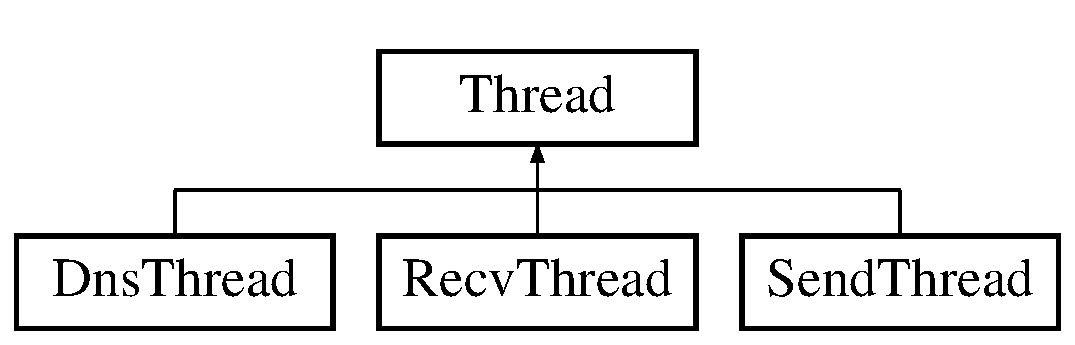
\includegraphics[height=2.000000cm]{class_thread}
\end{center}
\end{figure}
\subsection*{Public Member Functions}
\begin{DoxyCompactItemize}
\item 
\mbox{\Hypertarget{class_thread_a440c7d072fc8e81f5120fc3699f2bc0b}\label{class_thread_a440c7d072fc8e81f5120fc3699f2bc0b}} 
virtual \hyperlink{class_thread_a440c7d072fc8e81f5120fc3699f2bc0b}{$\sim$\+Thread} (void)
\begin{DoxyCompactList}\small\item\em 析构器 \end{DoxyCompactList}\item 
\mbox{\Hypertarget{class_thread_aa1ff0068d8e7ab1c8522827b89937611}\label{class_thread_aa1ff0068d8e7ab1c8522827b89937611}} 
void \hyperlink{class_thread_aa1ff0068d8e7ab1c8522827b89937611}{start} (void)
\begin{DoxyCompactList}\small\item\em 启动线程 \end{DoxyCompactList}\end{DoxyCompactItemize}


\subsection{Detailed Description}
线程 

The documentation for this class was generated from the following files\+:\begin{DoxyCompactItemize}
\item 
src/\hyperlink{_thread_8h}{Thread.\+h}\item 
src/\hyperlink{_thread_8cpp}{Thread.\+cpp}\end{DoxyCompactItemize}

\hypertarget{class_url_filter}{}\section{Url\+Filter Class Reference}
\label{class_url_filter}\index{Url\+Filter@{Url\+Filter}}


统一资源定位符过滤器接口  




{\ttfamily \#include $<$Url\+Filter.\+h$>$}

Inheritance diagram for Url\+Filter\+:\begin{figure}[H]
\begin{center}
\leavevmode
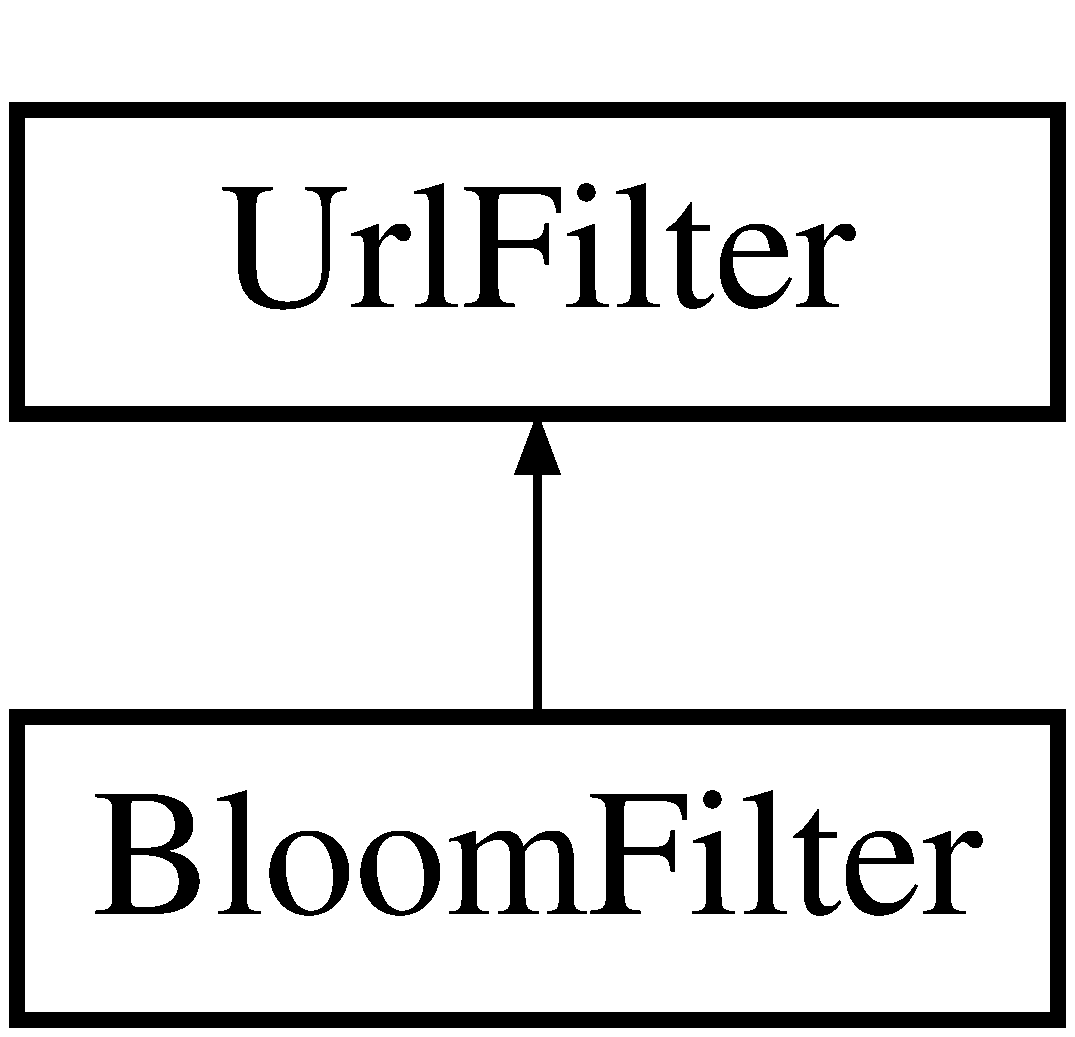
\includegraphics[height=2.000000cm]{class_url_filter}
\end{center}
\end{figure}
\subsection*{Public Member Functions}
\begin{DoxyCompactItemize}
\item 
\mbox{\Hypertarget{class_url_filter_ab6e4a890e83468c2717a89779c5dcc61}\label{class_url_filter_ab6e4a890e83468c2717a89779c5dcc61}} 
virtual \hyperlink{class_url_filter_ab6e4a890e83468c2717a89779c5dcc61}{$\sim$\+Url\+Filter} (void)
\begin{DoxyCompactList}\small\item\em 析构器 \end{DoxyCompactList}\item 
virtual bool \hyperlink{class_url_filter_a581b9ea03daefbf52344ceb3371f409a}{exist} (string const \&str\+Url)=0
\begin{DoxyCompactList}\small\item\em 判断某个统一资源定位符是否已经存在 \end{DoxyCompactList}\end{DoxyCompactItemize}


\subsection{Detailed Description}
统一资源定位符过滤器接口 

\subsection{Member Function Documentation}
\mbox{\Hypertarget{class_url_filter_a581b9ea03daefbf52344ceb3371f409a}\label{class_url_filter_a581b9ea03daefbf52344ceb3371f409a}} 
\index{Url\+Filter@{Url\+Filter}!exist@{exist}}
\index{exist@{exist}!Url\+Filter@{Url\+Filter}}
\subsubsection{\texorpdfstring{exist()}{exist()}}
{\footnotesize\ttfamily virtual bool Url\+Filter\+::exist (\begin{DoxyParamCaption}\item[{string const \&}]{str\+Url }\end{DoxyParamCaption})\hspace{0.3cm}{\ttfamily [pure virtual]}}



判断某个统一资源定位符是否已经存在 


\begin{DoxyRetVals}{Return values}
{\em true} & 存在 \\
\hline
{\em false} & 不存在 \\
\hline
\end{DoxyRetVals}
\begin{DoxyNote}{Note}
纯虚函数,子类根据不同过滤器的具体策略给出具体实现 
\end{DoxyNote}

\begin{DoxyParams}[1]{Parameters}
\mbox{\tt in}  & {\em str\+Url} & 统一资源定位符 \\
\hline
\end{DoxyParams}


Implemented in \hyperlink{class_bloom_filter_a78a992167b8efbc3be672469e68c5e97}{Bloom\+Filter}.



The documentation for this class was generated from the following file\+:\begin{DoxyCompactItemize}
\item 
src/\hyperlink{_url_filter_8h}{Url\+Filter.\+h}\end{DoxyCompactItemize}

\hypertarget{class_url_queues}{}\section{Url\+Queues Class Reference}
\label{class_url_queues}\index{Url\+Queues@{Url\+Queues}}


统一资源定位符队列  




{\ttfamily \#include $<$Url\+Queues.\+h$>$}

\subsection*{Public Member Functions}
\begin{DoxyCompactItemize}
\item 
\hyperlink{class_url_queues_a9761fc84cfd4bf6188a73229873fafd5}{Url\+Queues} (\hyperlink{class_url_filter}{Url\+Filter} \&filter)
\begin{DoxyCompactList}\small\item\em 构造器 \end{DoxyCompactList}\item 
\mbox{\Hypertarget{class_url_queues_aba370529b8c0cf49d068b1f5d5edafa0}\label{class_url_queues_aba370529b8c0cf49d068b1f5d5edafa0}} 
\hyperlink{class_url_queues_aba370529b8c0cf49d068b1f5d5edafa0}{$\sim$\+Url\+Queues} (void)
\begin{DoxyCompactList}\small\item\em 析构器 \end{DoxyCompactList}\item 
void \hyperlink{class_url_queues_a9649c30b72bdb4092732e505e4041e83}{push\+Raw\+Url} (\hyperlink{class_raw_url}{Raw\+Url} const \&raw\+Url)
\begin{DoxyCompactList}\small\item\em 压入原始统一资源定位符 \end{DoxyCompactList}\item 
\hyperlink{class_raw_url}{Raw\+Url} \hyperlink{class_url_queues_a8ceb4d6d67ce3b4afc7f0325ec254140}{pop\+Raw\+Url} (void)
\begin{DoxyCompactList}\small\item\em 弹出原始统一资源定位符 \end{DoxyCompactList}\item 
size\+\_\+t \hyperlink{class_url_queues_a713458484da28e9ada936ccc268413b3}{size\+Raw\+Url} (void) const
\begin{DoxyCompactList}\small\item\em 获取原始统一资源定位符数 \end{DoxyCompactList}\item 
bool \hyperlink{class_url_queues_af01992d66f4979e74e5c6661c76cbc1a}{empty\+Raw\+Url} (void) const
\begin{DoxyCompactList}\small\item\em 原始统一资源定位符队列空否 \end{DoxyCompactList}\item 
bool \hyperlink{class_url_queues_aaf6b48955b4ab667301188c48265506e}{full\+Raw\+Url} (void) const
\begin{DoxyCompactList}\small\item\em 原始统一资源定位符队列满否 \end{DoxyCompactList}\item 
\mbox{\Hypertarget{class_url_queues_a0b751864e21212cd2f8d8bf7b707507b}\label{class_url_queues_a0b751864e21212cd2f8d8bf7b707507b}} 
void \hyperlink{class_url_queues_a0b751864e21212cd2f8d8bf7b707507b}{clear\+Raw\+Url} (void)
\begin{DoxyCompactList}\small\item\em 清空原始统一资源定位符队列 \end{DoxyCompactList}\item 
void \hyperlink{class_url_queues_a4c7902b3c7ddd5c9758dbd0e5085ad18}{push\+Dns\+Url} (\hyperlink{class_dns_url}{Dns\+Url} const \&dns\+Url)
\begin{DoxyCompactList}\small\item\em 压入解析统一资源定位符 \end{DoxyCompactList}\item 
\hyperlink{class_dns_url}{Dns\+Url} \hyperlink{class_url_queues_ae42bc6d47ae51b0c02a0360f05bf0770}{pop\+Dns\+Url} (void)
\begin{DoxyCompactList}\small\item\em 弹出解析统一资源定位符 \end{DoxyCompactList}\item 
size\+\_\+t \hyperlink{class_url_queues_a65b094e4cd9f54ce9019b4045dd0e6da}{size\+Dns\+Url} (void) const
\begin{DoxyCompactList}\small\item\em 获取解析统一资源定位符数 \end{DoxyCompactList}\item 
bool \hyperlink{class_url_queues_adde4a7863750a113ba7e4da686bbf93c}{empty\+Dns\+Url} (void) const
\begin{DoxyCompactList}\small\item\em 解析统一资源定位符队列空否 \end{DoxyCompactList}\item 
bool \hyperlink{class_url_queues_a60ae6e63c4dcd998e0adfa9edf530509}{full\+Dns\+Url} (void) const
\begin{DoxyCompactList}\small\item\em 解析统一资源定位符队列满否 \end{DoxyCompactList}\item 
\mbox{\Hypertarget{class_url_queues_a136b3156b923cb0ceb7ef8577fd71d4f}\label{class_url_queues_a136b3156b923cb0ceb7ef8577fd71d4f}} 
void \hyperlink{class_url_queues_a136b3156b923cb0ceb7ef8577fd71d4f}{clear\+Dns\+Url} (void)
\begin{DoxyCompactList}\small\item\em 清空解析统一资源定位符队列 \end{DoxyCompactList}\item 
void \hyperlink{class_url_queues_a1f82f08afb7279075f3bef674b383bf4}{extract\+Url} (char const $\ast$html, \hyperlink{class_dns_url}{Dns\+Url} const \&dns\+Url)
\begin{DoxyCompactList}\small\item\em 从超文本标记语言页面内容中抽取统一资源定位符 \end{DoxyCompactList}\end{DoxyCompactItemize}


\subsection{Detailed Description}
统一资源定位符队列 

\subsection{Constructor \& Destructor Documentation}
\mbox{\Hypertarget{class_url_queues_a9761fc84cfd4bf6188a73229873fafd5}\label{class_url_queues_a9761fc84cfd4bf6188a73229873fafd5}} 
\index{Url\+Queues@{Url\+Queues}!Url\+Queues@{Url\+Queues}}
\index{Url\+Queues@{Url\+Queues}!Url\+Queues@{Url\+Queues}}
\subsubsection{\texorpdfstring{Url\+Queues()}{UrlQueues()}}
{\footnotesize\ttfamily Url\+Queues\+::\+Url\+Queues (\begin{DoxyParamCaption}\item[{\hyperlink{class_url_filter}{Url\+Filter} \&}]{filter }\end{DoxyParamCaption})}



构造器 


\begin{DoxyParams}[1]{Parameters}
\mbox{\tt in}  & {\em filter} & 统一资源定位符过滤器 \\
\hline
\end{DoxyParams}


\subsection{Member Function Documentation}
\mbox{\Hypertarget{class_url_queues_adde4a7863750a113ba7e4da686bbf93c}\label{class_url_queues_adde4a7863750a113ba7e4da686bbf93c}} 
\index{Url\+Queues@{Url\+Queues}!empty\+Dns\+Url@{empty\+Dns\+Url}}
\index{empty\+Dns\+Url@{empty\+Dns\+Url}!Url\+Queues@{Url\+Queues}}
\subsubsection{\texorpdfstring{empty\+Dns\+Url()}{emptyDnsUrl()}}
{\footnotesize\ttfamily bool Url\+Queues\+::empty\+Dns\+Url (\begin{DoxyParamCaption}\item[{void}]{ }\end{DoxyParamCaption}) const}



解析统一资源定位符队列空否 


\begin{DoxyRetVals}{Return values}
{\em true} & 空 \\
\hline
{\em false} & 不空 \\
\hline
\end{DoxyRetVals}
\mbox{\Hypertarget{class_url_queues_af01992d66f4979e74e5c6661c76cbc1a}\label{class_url_queues_af01992d66f4979e74e5c6661c76cbc1a}} 
\index{Url\+Queues@{Url\+Queues}!empty\+Raw\+Url@{empty\+Raw\+Url}}
\index{empty\+Raw\+Url@{empty\+Raw\+Url}!Url\+Queues@{Url\+Queues}}
\subsubsection{\texorpdfstring{empty\+Raw\+Url()}{emptyRawUrl()}}
{\footnotesize\ttfamily bool Url\+Queues\+::empty\+Raw\+Url (\begin{DoxyParamCaption}\item[{void}]{ }\end{DoxyParamCaption}) const}



原始统一资源定位符队列空否 


\begin{DoxyRetVals}{Return values}
{\em true} & 空 \\
\hline
{\em false} & 不空\\
\hline
\end{DoxyRetVals}
原始统一资源定位符队列空否 空返回true,不空返回false \mbox{\Hypertarget{class_url_queues_a1f82f08afb7279075f3bef674b383bf4}\label{class_url_queues_a1f82f08afb7279075f3bef674b383bf4}} 
\index{Url\+Queues@{Url\+Queues}!extract\+Url@{extract\+Url}}
\index{extract\+Url@{extract\+Url}!Url\+Queues@{Url\+Queues}}
\subsubsection{\texorpdfstring{extract\+Url()}{extractUrl()}}
{\footnotesize\ttfamily void Url\+Queues\+::extract\+Url (\begin{DoxyParamCaption}\item[{char const $\ast$}]{html,  }\item[{\hyperlink{class_dns_url}{Dns\+Url} const \&}]{dns\+Url }\end{DoxyParamCaption})}



从超文本标记语言页面内容中抽取统一资源定位符 


\begin{DoxyParams}[1]{Parameters}
\mbox{\tt in}  & {\em html} & 超文本标记语言页面内容字符串 \\
\hline
\mbox{\tt in}  & {\em dns\+Url} & 被抽取页面解析统一资源定位符 \\
\hline
\end{DoxyParams}
\mbox{\Hypertarget{class_url_queues_a60ae6e63c4dcd998e0adfa9edf530509}\label{class_url_queues_a60ae6e63c4dcd998e0adfa9edf530509}} 
\index{Url\+Queues@{Url\+Queues}!full\+Dns\+Url@{full\+Dns\+Url}}
\index{full\+Dns\+Url@{full\+Dns\+Url}!Url\+Queues@{Url\+Queues}}
\subsubsection{\texorpdfstring{full\+Dns\+Url()}{fullDnsUrl()}}
{\footnotesize\ttfamily bool Url\+Queues\+::full\+Dns\+Url (\begin{DoxyParamCaption}\item[{void}]{ }\end{DoxyParamCaption}) const}



解析统一资源定位符队列满否 


\begin{DoxyRetVals}{Return values}
{\em true} & 满 \\
\hline
{\em false} & 不满 \\
\hline
\end{DoxyRetVals}
\mbox{\Hypertarget{class_url_queues_aaf6b48955b4ab667301188c48265506e}\label{class_url_queues_aaf6b48955b4ab667301188c48265506e}} 
\index{Url\+Queues@{Url\+Queues}!full\+Raw\+Url@{full\+Raw\+Url}}
\index{full\+Raw\+Url@{full\+Raw\+Url}!Url\+Queues@{Url\+Queues}}
\subsubsection{\texorpdfstring{full\+Raw\+Url()}{fullRawUrl()}}
{\footnotesize\ttfamily bool Url\+Queues\+::full\+Raw\+Url (\begin{DoxyParamCaption}\item[{void}]{ }\end{DoxyParamCaption}) const}



原始统一资源定位符队列满否 


\begin{DoxyRetVals}{Return values}
{\em true} & 满 \\
\hline
{\em false} & 不满 \\
\hline
\end{DoxyRetVals}
\mbox{\Hypertarget{class_url_queues_ae42bc6d47ae51b0c02a0360f05bf0770}\label{class_url_queues_ae42bc6d47ae51b0c02a0360f05bf0770}} 
\index{Url\+Queues@{Url\+Queues}!pop\+Dns\+Url@{pop\+Dns\+Url}}
\index{pop\+Dns\+Url@{pop\+Dns\+Url}!Url\+Queues@{Url\+Queues}}
\subsubsection{\texorpdfstring{pop\+Dns\+Url()}{popDnsUrl()}}
{\footnotesize\ttfamily \hyperlink{class_dns_url}{Dns\+Url} Url\+Queues\+::pop\+Dns\+Url (\begin{DoxyParamCaption}\item[{void}]{ }\end{DoxyParamCaption})}



弹出解析统一资源定位符 

\begin{DoxyReturn}{Returns}
解析统一资源定位符 
\end{DoxyReturn}
\mbox{\Hypertarget{class_url_queues_a8ceb4d6d67ce3b4afc7f0325ec254140}\label{class_url_queues_a8ceb4d6d67ce3b4afc7f0325ec254140}} 
\index{Url\+Queues@{Url\+Queues}!pop\+Raw\+Url@{pop\+Raw\+Url}}
\index{pop\+Raw\+Url@{pop\+Raw\+Url}!Url\+Queues@{Url\+Queues}}
\subsubsection{\texorpdfstring{pop\+Raw\+Url()}{popRawUrl()}}
{\footnotesize\ttfamily \hyperlink{class_raw_url}{Raw\+Url} Url\+Queues\+::pop\+Raw\+Url (\begin{DoxyParamCaption}\item[{void}]{ }\end{DoxyParamCaption})}



弹出原始统一资源定位符 

\begin{DoxyReturn}{Returns}
原始统一资源定位符 
\end{DoxyReturn}
\mbox{\Hypertarget{class_url_queues_a4c7902b3c7ddd5c9758dbd0e5085ad18}\label{class_url_queues_a4c7902b3c7ddd5c9758dbd0e5085ad18}} 
\index{Url\+Queues@{Url\+Queues}!push\+Dns\+Url@{push\+Dns\+Url}}
\index{push\+Dns\+Url@{push\+Dns\+Url}!Url\+Queues@{Url\+Queues}}
\subsubsection{\texorpdfstring{push\+Dns\+Url()}{pushDnsUrl()}}
{\footnotesize\ttfamily void Url\+Queues\+::push\+Dns\+Url (\begin{DoxyParamCaption}\item[{\hyperlink{class_dns_url}{Dns\+Url} const \&}]{dns\+Url }\end{DoxyParamCaption})}



压入解析统一资源定位符 


\begin{DoxyParams}[1]{Parameters}
\mbox{\tt in}  & {\em dns\+Url} & 解析统一资源定位符 \\
\hline
\end{DoxyParams}
\mbox{\Hypertarget{class_url_queues_a9649c30b72bdb4092732e505e4041e83}\label{class_url_queues_a9649c30b72bdb4092732e505e4041e83}} 
\index{Url\+Queues@{Url\+Queues}!push\+Raw\+Url@{push\+Raw\+Url}}
\index{push\+Raw\+Url@{push\+Raw\+Url}!Url\+Queues@{Url\+Queues}}
\subsubsection{\texorpdfstring{push\+Raw\+Url()}{pushRawUrl()}}
{\footnotesize\ttfamily void Url\+Queues\+::push\+Raw\+Url (\begin{DoxyParamCaption}\item[{\hyperlink{class_raw_url}{Raw\+Url} const \&}]{raw\+Url }\end{DoxyParamCaption})}



压入原始统一资源定位符 


\begin{DoxyParams}[1]{Parameters}
\mbox{\tt in}  & {\em raw\+Url} & 原始统一资源定位符 \\
\hline
\end{DoxyParams}
\mbox{\Hypertarget{class_url_queues_a65b094e4cd9f54ce9019b4045dd0e6da}\label{class_url_queues_a65b094e4cd9f54ce9019b4045dd0e6da}} 
\index{Url\+Queues@{Url\+Queues}!size\+Dns\+Url@{size\+Dns\+Url}}
\index{size\+Dns\+Url@{size\+Dns\+Url}!Url\+Queues@{Url\+Queues}}
\subsubsection{\texorpdfstring{size\+Dns\+Url()}{sizeDnsUrl()}}
{\footnotesize\ttfamily size\+\_\+t Url\+Queues\+::size\+Dns\+Url (\begin{DoxyParamCaption}\item[{void}]{ }\end{DoxyParamCaption}) const}



获取解析统一资源定位符数 

\begin{DoxyReturn}{Returns}
解析统一资源定位符数 
\end{DoxyReturn}
\mbox{\Hypertarget{class_url_queues_a713458484da28e9ada936ccc268413b3}\label{class_url_queues_a713458484da28e9ada936ccc268413b3}} 
\index{Url\+Queues@{Url\+Queues}!size\+Raw\+Url@{size\+Raw\+Url}}
\index{size\+Raw\+Url@{size\+Raw\+Url}!Url\+Queues@{Url\+Queues}}
\subsubsection{\texorpdfstring{size\+Raw\+Url()}{sizeRawUrl()}}
{\footnotesize\ttfamily size\+\_\+t Url\+Queues\+::size\+Raw\+Url (\begin{DoxyParamCaption}\item[{void}]{ }\end{DoxyParamCaption}) const}



获取原始统一资源定位符数 

\begin{DoxyReturn}{Returns}
原始统一资源定位符数 
\end{DoxyReturn}


The documentation for this class was generated from the following files\+:\begin{DoxyCompactItemize}
\item 
src/\hyperlink{_url_queues_8h}{Url\+Queues.\+h}\item 
src/\hyperlink{_url_queues_8cpp}{Url\+Queues.\+cpp}\end{DoxyCompactItemize}

\hypertarget{class_web_crawler}{}\section{Web\+Crawler Class Reference}
\label{class_web_crawler}\index{Web\+Crawler@{Web\+Crawler}}


网络爬虫  




{\ttfamily \#include $<$Web\+Crawler.\+h$>$}

\subsection*{Public Member Functions}
\begin{DoxyCompactItemize}
\item 
\hyperlink{class_web_crawler_ad8120b764c991bbf51764d47ea097b88}{Web\+Crawler} (\hyperlink{class_url_filter}{Url\+Filter} \&filter)
\begin{DoxyCompactList}\small\item\em 构造器 \end{DoxyCompactList}\item 
\mbox{\Hypertarget{class_web_crawler_a4f135eede21f8a08df3b4b86e7928f7b}\label{class_web_crawler_a4f135eede21f8a08df3b4b86e7928f7b}} 
\hyperlink{class_web_crawler_a4f135eede21f8a08df3b4b86e7928f7b}{$\sim$\+Web\+Crawler} (void)
\begin{DoxyCompactList}\small\item\em 析构器 \end{DoxyCompactList}\item 
void \hyperlink{class_web_crawler_aa33817c1f415d3be793e7b43198d253e}{init} (bool daemon=false)
\begin{DoxyCompactList}\small\item\em 初始化 \end{DoxyCompactList}\item 
\mbox{\Hypertarget{class_web_crawler_a940428b71b32361953b241079c62b24d}\label{class_web_crawler_a940428b71b32361953b241079c62b24d}} 
void \hyperlink{class_web_crawler_a940428b71b32361953b241079c62b24d}{exec} (void)
\begin{DoxyCompactList}\small\item\em 执行多路输入输出循环 \end{DoxyCompactList}\item 
\mbox{\Hypertarget{class_web_crawler_a6d21283f301038ee6aa5bc1bb57d1d7c}\label{class_web_crawler_a6d21283f301038ee6aa5bc1bb57d1d7c}} 
void \hyperlink{class_web_crawler_a6d21283f301038ee6aa5bc1bb57d1d7c}{start\+Job} (void)
\begin{DoxyCompactList}\small\item\em 启动一个抓取任务 \end{DoxyCompactList}\item 
void \hyperlink{class_web_crawler_a7da15941a0fd20e1ae53d4077d61c9d4}{stop\+Job} (bool success=true)
\begin{DoxyCompactList}\small\item\em 停止一个抓取任务 \end{DoxyCompactList}\end{DoxyCompactItemize}
\subsection*{Public Attributes}
\begin{DoxyCompactItemize}
\item 
\mbox{\Hypertarget{class_web_crawler_a94412c52ed3992adfb0195c0075e5e06}\label{class_web_crawler_a94412c52ed3992adfb0195c0075e5e06}} 
\hyperlink{class_log}{Log} \hyperlink{class_web_crawler_a94412c52ed3992adfb0195c0075e5e06}{m\+\_\+log}
\begin{DoxyCompactList}\small\item\em 日志 \end{DoxyCompactList}\item 
\mbox{\Hypertarget{class_web_crawler_a02271762fedba90a0b00f8be65423de4}\label{class_web_crawler_a02271762fedba90a0b00f8be65423de4}} 
\hyperlink{class_configurator}{Configurator} \hyperlink{class_web_crawler_a02271762fedba90a0b00f8be65423de4}{m\+\_\+cfg}
\begin{DoxyCompactList}\small\item\em 配置器 \end{DoxyCompactList}\item 
\mbox{\Hypertarget{class_web_crawler_a8492c84e209f4cbf733e939dd5cd5317}\label{class_web_crawler_a8492c84e209f4cbf733e939dd5cd5317}} 
\hyperlink{class_multi_io}{Multi\+Io} \hyperlink{class_web_crawler_a8492c84e209f4cbf733e939dd5cd5317}{m\+\_\+multi\+Io}
\begin{DoxyCompactList}\small\item\em 多路输入输出 \end{DoxyCompactList}\item 
\mbox{\Hypertarget{class_web_crawler_af9ff344fb9447d40a32e40435882a075}\label{class_web_crawler_af9ff344fb9447d40a32e40435882a075}} 
\hyperlink{class_plugin_mngr}{Plugin\+Mngr} \hyperlink{class_web_crawler_af9ff344fb9447d40a32e40435882a075}{m\+\_\+plugin\+Mngr}
\begin{DoxyCompactList}\small\item\em 插件管理器 \end{DoxyCompactList}\item 
\mbox{\Hypertarget{class_web_crawler_ab9a440531fbd41b43b4dd97654000dae}\label{class_web_crawler_ab9a440531fbd41b43b4dd97654000dae}} 
\hyperlink{class_url_queues}{Url\+Queues} \hyperlink{class_web_crawler_ab9a440531fbd41b43b4dd97654000dae}{m\+\_\+url\+Queues}
\begin{DoxyCompactList}\small\item\em 统一资源定位符队列 \end{DoxyCompactList}\item 
\mbox{\Hypertarget{class_web_crawler_ada21f95fb073ea1f81c8c7853ace9c6e}\label{class_web_crawler_ada21f95fb073ea1f81c8c7853ace9c6e}} 
\hyperlink{class_dns_thread}{Dns\+Thread} \hyperlink{class_web_crawler_ada21f95fb073ea1f81c8c7853ace9c6e}{m\+\_\+dns\+Thread}
\begin{DoxyCompactList}\small\item\em 域名解析线程 \end{DoxyCompactList}\item 
\mbox{\Hypertarget{class_web_crawler_ae5098d623339f79eaaf7dd5b69d64a60}\label{class_web_crawler_ae5098d623339f79eaaf7dd5b69d64a60}} 
\hyperlink{class_send_thread}{Send\+Thread} \hyperlink{class_web_crawler_ae5098d623339f79eaaf7dd5b69d64a60}{m\+\_\+send\+Thread}
\begin{DoxyCompactList}\small\item\em 发送线程 \end{DoxyCompactList}\end{DoxyCompactItemize}


\subsection{Detailed Description}
网络爬虫 

\subsection{Constructor \& Destructor Documentation}
\mbox{\Hypertarget{class_web_crawler_ad8120b764c991bbf51764d47ea097b88}\label{class_web_crawler_ad8120b764c991bbf51764d47ea097b88}} 
\index{Web\+Crawler@{Web\+Crawler}!Web\+Crawler@{Web\+Crawler}}
\index{Web\+Crawler@{Web\+Crawler}!Web\+Crawler@{Web\+Crawler}}
\subsubsection{\texorpdfstring{Web\+Crawler()}{WebCrawler()}}
{\footnotesize\ttfamily Web\+Crawler\+::\+Web\+Crawler (\begin{DoxyParamCaption}\item[{\hyperlink{class_url_filter}{Url\+Filter} \&}]{filter }\end{DoxyParamCaption})}



构造器 


\begin{DoxyParams}[1]{Parameters}
\mbox{\tt in}  & {\em filter} & 统一资源定位符过滤器 \\
\hline
\end{DoxyParams}


\subsection{Member Function Documentation}
\mbox{\Hypertarget{class_web_crawler_aa33817c1f415d3be793e7b43198d253e}\label{class_web_crawler_aa33817c1f415d3be793e7b43198d253e}} 
\index{Web\+Crawler@{Web\+Crawler}!init@{init}}
\index{init@{init}!Web\+Crawler@{Web\+Crawler}}
\subsubsection{\texorpdfstring{init()}{init()}}
{\footnotesize\ttfamily void Web\+Crawler\+::init (\begin{DoxyParamCaption}\item[{bool}]{daemon = {\ttfamily false} }\end{DoxyParamCaption})}



初始化 


\begin{DoxyParams}[1]{Parameters}
\mbox{\tt in}  & {\em daemon} & 是否以精灵进程方式运行 \\
\hline
\end{DoxyParams}
\mbox{\Hypertarget{class_web_crawler_a7da15941a0fd20e1ae53d4077d61c9d4}\label{class_web_crawler_a7da15941a0fd20e1ae53d4077d61c9d4}} 
\index{Web\+Crawler@{Web\+Crawler}!stop\+Job@{stop\+Job}}
\index{stop\+Job@{stop\+Job}!Web\+Crawler@{Web\+Crawler}}
\subsubsection{\texorpdfstring{stop\+Job()}{stopJob()}}
{\footnotesize\ttfamily void Web\+Crawler\+::stop\+Job (\begin{DoxyParamCaption}\item[{bool}]{success = {\ttfamily true} }\end{DoxyParamCaption})}



停止一个抓取任务 


\begin{DoxyParams}[1]{Parameters}
\mbox{\tt in}  & {\em success} & 是否成功 \\
\hline
\end{DoxyParams}


The documentation for this class was generated from the following files\+:\begin{DoxyCompactItemize}
\item 
src/\hyperlink{_web_crawler_8h}{Web\+Crawler.\+h}\item 
src/\hyperlink{_web_crawler_8cpp}{Web\+Crawler.\+cpp}\end{DoxyCompactItemize}

\chapter{File Documentation}
\hypertarget{_bloom_filter_8cpp}{}\section{src/\+Bloom\+Filter.cpp File Reference}
\label{_bloom_filter_8cpp}\index{src/\+Bloom\+Filter.\+cpp@{src/\+Bloom\+Filter.\+cpp}}


实现\+::\+Bloom\+Filter类  


{\ttfamily \#include \char`\"{}Precompile.\+h\char`\"{}}\newline
{\ttfamily \#include \char`\"{}Web\+Crawler.\+h\char`\"{}}\newline
{\ttfamily \#include \char`\"{}Bloom\+Filter.\+h\char`\"{}}\newline


\subsection{Detailed Description}
实现\+::\+Bloom\+Filter类 

\begin{DoxyAuthor}{Author}
闵卫 
\end{DoxyAuthor}
\begin{DoxyDate}{Date}
2015年11月20日 
\end{DoxyDate}
\begin{DoxyVersion}{Version}
1.\+0.\+0.\+1 
\end{DoxyVersion}

\hypertarget{_bloom_filter_8h}{}\section{src/\+Bloom\+Filter.h File Reference}
\label{_bloom_filter_8h}\index{src/\+Bloom\+Filter.\+h@{src/\+Bloom\+Filter.\+h}}


声明\+::\+Bloom\+Filter类  


{\ttfamily \#include \char`\"{}Url\+Filter.\+h\char`\"{}}\newline
{\ttfamily \#include \char`\"{}Hash.\+h\char`\"{}}\newline
\subsection*{Classes}
\begin{DoxyCompactItemize}
\item 
class \hyperlink{class_bloom_filter}{Bloom\+Filter}
\begin{DoxyCompactList}\small\item\em 布隆过滤器 \end{DoxyCompactList}\end{DoxyCompactItemize}


\subsection{Detailed Description}
声明\+::\+Bloom\+Filter类 

\begin{DoxyAuthor}{Author}
闵卫 
\end{DoxyAuthor}
\begin{DoxyDate}{Date}
2015年11月20日 
\end{DoxyDate}
\begin{DoxyVersion}{Version}
1.\+0.\+0.\+1 
\end{DoxyVersion}

\hypertarget{_configurator_8cpp}{}\section{src/\+Configurator.cpp File Reference}
\label{_configurator_8cpp}\index{src/\+Configurator.\+cpp@{src/\+Configurator.\+cpp}}


实现\+::\+Configurator类  


{\ttfamily \#include \char`\"{}Precompile.\+h\char`\"{}}\newline
{\ttfamily \#include \char`\"{}Web\+Crawler.\+h\char`\"{}}\newline
{\ttfamily \#include \char`\"{}Str\+Kit.\+h\char`\"{}}\newline


\subsection{Detailed Description}
实现\+::\+Configurator类 

\begin{DoxyAuthor}{Author}
闵卫 
\end{DoxyAuthor}
\begin{DoxyDate}{Date}
2015年11月20日 
\end{DoxyDate}
\begin{DoxyVersion}{Version}
1.\+0.\+0.\+1 
\end{DoxyVersion}

\hypertarget{_configurator_8h}{}\section{src/\+Configurator.h File Reference}
\label{_configurator_8h}\index{src/\+Configurator.\+h@{src/\+Configurator.\+h}}


声明\+::\+Configurator类  


\subsection*{Classes}
\begin{DoxyCompactItemize}
\item 
class \hyperlink{class_configurator}{Configurator}
\begin{DoxyCompactList}\small\item\em 配置器 \end{DoxyCompactList}\end{DoxyCompactItemize}


\subsection{Detailed Description}
声明\+::\+Configurator类 

\begin{DoxyAuthor}{Author}
闵卫 
\end{DoxyAuthor}
\begin{DoxyDate}{Date}
2015年11月20日 
\end{DoxyDate}
\begin{DoxyVersion}{Version}
1.\+0.\+0.\+1 
\end{DoxyVersion}

\hypertarget{_dns_thread_8cpp}{}\section{src/\+Dns\+Thread.cpp File Reference}
\label{_dns_thread_8cpp}\index{src/\+Dns\+Thread.\+cpp@{src/\+Dns\+Thread.\+cpp}}


实现\+::\+Dns\+Thread类  


{\ttfamily \#include \char`\"{}Precompile.\+h\char`\"{}}\newline
{\ttfamily \#include \char`\"{}Web\+Crawler.\+h\char`\"{}}\newline


\subsection{Detailed Description}
实现\+::\+Dns\+Thread类 

\begin{DoxyAuthor}{Author}
闵卫 
\end{DoxyAuthor}
\begin{DoxyDate}{Date}
2015年11月20日 
\end{DoxyDate}
\begin{DoxyVersion}{Version}
1.\+0.\+0.\+1 
\end{DoxyVersion}

\hypertarget{_dns_thread_8h}{}\section{src/\+Dns\+Thread.h File Reference}
\label{_dns_thread_8h}\index{src/\+Dns\+Thread.\+h@{src/\+Dns\+Thread.\+h}}


声明\+::\+Dns\+Thread类  


{\ttfamily \#include \char`\"{}Thread.\+h\char`\"{}}\newline
\subsection*{Classes}
\begin{DoxyCompactItemize}
\item 
class \hyperlink{class_dns_thread}{Dns\+Thread}
\begin{DoxyCompactList}\small\item\em 域名解析线程 \end{DoxyCompactList}\end{DoxyCompactItemize}


\subsection{Detailed Description}
声明\+::\+Dns\+Thread类 

\begin{DoxyAuthor}{Author}
闵卫 
\end{DoxyAuthor}
\begin{DoxyDate}{Date}
2015年11月20日 
\end{DoxyDate}
\begin{DoxyVersion}{Version}
1.\+0.\+0.\+1 
\end{DoxyVersion}

\hypertarget{_hash_8cpp}{}\section{src/\+Hash.cpp File Reference}
\label{_hash_8cpp}\index{src/\+Hash.\+cpp@{src/\+Hash.\+cpp}}


实现\+::\+Hash类  


{\ttfamily \#include \char`\"{}Precompile.\+h\char`\"{}}\newline
{\ttfamily \#include \char`\"{}Hash.\+h\char`\"{}}\newline


\subsection{Detailed Description}
实现\+::\+Hash类 

\begin{DoxyAuthor}{Author}
闵卫 
\end{DoxyAuthor}
\begin{DoxyDate}{Date}
2015年11月20日 
\end{DoxyDate}
\begin{DoxyVersion}{Version}
1.\+0.\+0.\+1 
\end{DoxyVersion}

\hypertarget{_hash_8h}{}\section{src/\+Hash.h File Reference}
\label{_hash_8h}\index{src/\+Hash.\+h@{src/\+Hash.\+h}}


声明\+::\+Hash类  


\subsection*{Classes}
\begin{DoxyCompactItemize}
\item 
class \hyperlink{class_hash}{Hash}
\begin{DoxyCompactList}\small\item\em 哈希器 \end{DoxyCompactList}\end{DoxyCompactItemize}


\subsection{Detailed Description}
声明\+::\+Hash类 

\begin{DoxyAuthor}{Author}
闵卫 
\end{DoxyAuthor}
\begin{DoxyDate}{Date}
2015年11月20日 
\end{DoxyDate}
\begin{DoxyVersion}{Version}
1.\+0.\+0.\+1 
\end{DoxyVersion}

\hypertarget{_http_8h}{}\section{src/\+Http.h File Reference}
\label{_http_8h}\index{src/\+Http.\+h@{src/\+Http.\+h}}


定义\+::\+Http\+Header类和\+::\+Http\+Response类  


{\ttfamily \#include \char`\"{}Url.\+h\char`\"{}}\newline
\subsection*{Classes}
\begin{DoxyCompactItemize}
\item 
class \hyperlink{class_http_header}{Http\+Header}
\begin{DoxyCompactList}\small\item\em 超文本传输协议响应包头 \end{DoxyCompactList}\item 
class \hyperlink{class_http_response}{Http\+Response}
\begin{DoxyCompactList}\small\item\em 超文本传输协议响应 \end{DoxyCompactList}\end{DoxyCompactItemize}


\subsection{Detailed Description}
定义\+::\+Http\+Header类和\+::\+Http\+Response类 

\begin{DoxyAuthor}{Author}
闵卫 
\end{DoxyAuthor}
\begin{DoxyDate}{Date}
2015年11月20日 
\end{DoxyDate}
\begin{DoxyVersion}{Version}
1.\+0.\+0.\+1 
\end{DoxyVersion}

\hypertarget{_log_8cpp}{}\section{src/\+Log.cpp File Reference}
\label{_log_8cpp}\index{src/\+Log.\+cpp@{src/\+Log.\+cpp}}


实现\+::\+Log类  


{\ttfamily \#include \char`\"{}Precompile.\+h\char`\"{}}\newline
{\ttfamily \#include \char`\"{}Web\+Crawler.\+h\char`\"{}}\newline


\subsection{Detailed Description}
实现\+::\+Log类 

\begin{DoxyAuthor}{Author}
闵卫 
\end{DoxyAuthor}
\begin{DoxyDate}{Date}
2015年11月20日 
\end{DoxyDate}
\begin{DoxyVersion}{Version}
1.\+0.\+0.\+1 
\end{DoxyVersion}

\hypertarget{_log_8h}{}\section{src/\+Log.h File Reference}
\label{_log_8h}\index{src/\+Log.\+h@{src/\+Log.\+h}}


声明\+::\+Log类  


\subsection*{Classes}
\begin{DoxyCompactItemize}
\item 
class \hyperlink{class_log}{Log}
\begin{DoxyCompactList}\small\item\em 日志 \end{DoxyCompactList}\end{DoxyCompactItemize}


\subsection{Detailed Description}
声明\+::\+Log类 

\begin{DoxyAuthor}{Author}
闵卫 
\end{DoxyAuthor}
\begin{DoxyDate}{Date}
2015年11月20日 
\end{DoxyDate}
\begin{DoxyVersion}{Version}
1.\+0.\+0.\+1 
\end{DoxyVersion}

\hypertarget{_main_8cpp}{}\section{src/\+Main.cpp File Reference}
\label{_main_8cpp}\index{src/\+Main.\+cpp@{src/\+Main.\+cpp}}


定义\+::main函数  


{\ttfamily \#include \char`\"{}Precompile.\+h\char`\"{}}\newline
{\ttfamily \#include \char`\"{}Web\+Crawler.\+h\char`\"{}}\newline
{\ttfamily \#include \char`\"{}Bloom\+Filter.\+h\char`\"{}}\newline
\subsection*{Functions}
\begin{DoxyCompactItemize}
\item 
int \hyperlink{_main_8cpp_a0ddf1224851353fc92bfbff6f499fa97}{main} (int argc, char $\ast$argv\mbox{[}$\,$\mbox{]})
\begin{DoxyCompactList}\small\item\em 进程入口函数 \end{DoxyCompactList}\end{DoxyCompactItemize}
\subsection*{Variables}
\begin{DoxyCompactItemize}
\item 
\mbox{\Hypertarget{_main_8cpp_aec5109baf80c5e8540aad9d2a6ba1566}\label{_main_8cpp_aec5109baf80c5e8540aad9d2a6ba1566}} 
\hyperlink{class_bloom_filter}{Bloom\+Filter} {\bfseries g\+\_\+filter}
\item 
\mbox{\Hypertarget{_main_8cpp_a8e826eac7119c7ebc0db05cdef6812c7}\label{_main_8cpp_a8e826eac7119c7ebc0db05cdef6812c7}} 
\hyperlink{class_web_crawler}{Web\+Crawler} $\ast$ \hyperlink{_main_8cpp_a8e826eac7119c7ebc0db05cdef6812c7}{g\+\_\+app} = new \hyperlink{class_web_crawler}{Web\+Crawler} (g\+\_\+filter)
\begin{DoxyCompactList}\small\item\em 应用程序对象 \end{DoxyCompactList}\end{DoxyCompactItemize}


\subsection{Detailed Description}
定义\+::main函数 

\begin{DoxyAuthor}{Author}
闵卫 
\end{DoxyAuthor}
\begin{DoxyDate}{Date}
2015年11月20日 
\end{DoxyDate}
\begin{DoxyVersion}{Version}
1.\+0.\+0.\+1 
\end{DoxyVersion}


\subsection{Function Documentation}
\mbox{\Hypertarget{_main_8cpp_a0ddf1224851353fc92bfbff6f499fa97}\label{_main_8cpp_a0ddf1224851353fc92bfbff6f499fa97}} 
\index{Main.\+cpp@{Main.\+cpp}!main@{main}}
\index{main@{main}!Main.\+cpp@{Main.\+cpp}}
\subsubsection{\texorpdfstring{main()}{main()}}
{\footnotesize\ttfamily int main (\begin{DoxyParamCaption}\item[{int}]{argc,  }\item[{char $\ast$}]{argv\mbox{[}$\,$\mbox{]} }\end{DoxyParamCaption})}



进程入口函数 


\begin{DoxyRetVals}{Return values}
{\em E\+X\+I\+T\+\_\+\+S\+U\+C\+C\+E\+SS} & 进程成功退出 \\
\hline
{\em E\+X\+I\+T\+\_\+\+F\+A\+I\+L\+U\+RE} & 进程失败退出 \\
\hline
\end{DoxyRetVals}

\begin{DoxyParams}[1]{Parameters}
\mbox{\tt in}  & {\em argc} & 命令行参数个数 \\
\hline
\mbox{\tt in}  & {\em argv} & 命令行参数列表 \\
\hline
\end{DoxyParams}

\hypertarget{_multi_io_8cpp}{}\section{src/\+Multi\+Io.cpp File Reference}
\label{_multi_io_8cpp}\index{src/\+Multi\+Io.\+cpp@{src/\+Multi\+Io.\+cpp}}


实现\+::\+Multi\+Io类  


{\ttfamily \#include \char`\"{}Precompile.\+h\char`\"{}}\newline
{\ttfamily \#include \char`\"{}Web\+Crawler.\+h\char`\"{}}\newline


\subsection{Detailed Description}
实现\+::\+Multi\+Io类 

\begin{DoxyAuthor}{Author}
闵卫 
\end{DoxyAuthor}
\begin{DoxyDate}{Date}
2015年11月20日 
\end{DoxyDate}
\begin{DoxyVersion}{Version}
1.\+0.\+0.\+1 
\end{DoxyVersion}

\hypertarget{_multi_io_8h}{}\section{src/\+Multi\+Io.h File Reference}
\label{_multi_io_8h}\index{src/\+Multi\+Io.\+h@{src/\+Multi\+Io.\+h}}


声明\+::\+Multi\+Io类  


\subsection*{Classes}
\begin{DoxyCompactItemize}
\item 
class \hyperlink{class_multi_io}{Multi\+Io}
\begin{DoxyCompactList}\small\item\em 多路输入输出 \end{DoxyCompactList}\end{DoxyCompactItemize}


\subsection{Detailed Description}
声明\+::\+Multi\+Io类 

\begin{DoxyAuthor}{Author}
闵卫 
\end{DoxyAuthor}
\begin{DoxyDate}{Date}
2015年11月20日 
\end{DoxyDate}
\begin{DoxyVersion}{Version}
1.\+0.\+0.\+1 
\end{DoxyVersion}

\hypertarget{_plugin_8h}{}\section{src/\+Plugin.h File Reference}
\label{_plugin_8h}\index{src/\+Plugin.\+h@{src/\+Plugin.\+h}}


定义\+::\+Plugin接口类  


\subsection*{Classes}
\begin{DoxyCompactItemize}
\item 
class \hyperlink{class_plugin}{Plugin}
\begin{DoxyCompactList}\small\item\em 插件接口 \end{DoxyCompactList}\end{DoxyCompactItemize}


\subsection{Detailed Description}
定义\+::\+Plugin接口类 

\begin{DoxyAuthor}{Author}
闵卫 
\end{DoxyAuthor}
\begin{DoxyDate}{Date}
2015年11月20日 
\end{DoxyDate}
\begin{DoxyVersion}{Version}
1.\+0.\+0.\+1 
\end{DoxyVersion}

\hypertarget{_plugin_mngr_8cpp}{}\section{src/\+Plugin\+Mngr.cpp File Reference}
\label{_plugin_mngr_8cpp}\index{src/\+Plugin\+Mngr.\+cpp@{src/\+Plugin\+Mngr.\+cpp}}


实现\+::\+Plugin\+Mngr类  


{\ttfamily \#include \char`\"{}Precompile.\+h\char`\"{}}\newline
{\ttfamily \#include \char`\"{}Web\+Crawler.\+h\char`\"{}}\newline
{\ttfamily \#include \char`\"{}Plugin.\+h\char`\"{}}\newline
{\ttfamily \#include \char`\"{}Str\+Kit.\+h\char`\"{}}\newline


\subsection{Detailed Description}
实现\+::\+Plugin\+Mngr类 

\begin{DoxyAuthor}{Author}
闵卫 
\end{DoxyAuthor}
\begin{DoxyDate}{Date}
2015年11月20日 
\end{DoxyDate}
\begin{DoxyVersion}{Version}
1.\+0.\+0.\+1 
\end{DoxyVersion}

\hypertarget{_plugin_mngr_8h}{}\section{src/\+Plugin\+Mngr.h File Reference}
\label{_plugin_mngr_8h}\index{src/\+Plugin\+Mngr.\+h@{src/\+Plugin\+Mngr.\+h}}


声明\+::\+Plugin\+Mngr类  


\subsection*{Classes}
\begin{DoxyCompactItemize}
\item 
class \hyperlink{class_plugin_mngr}{Plugin\+Mngr}
\begin{DoxyCompactList}\small\item\em 插件管理器 \end{DoxyCompactList}\end{DoxyCompactItemize}


\subsection{Detailed Description}
声明\+::\+Plugin\+Mngr类 

\begin{DoxyAuthor}{Author}
闵卫 
\end{DoxyAuthor}
\begin{DoxyDate}{Date}
2015年11月20日 
\end{DoxyDate}
\begin{DoxyVersion}{Version}
1.\+0.\+0.\+1 
\end{DoxyVersion}

\hypertarget{_precompile_8h}{}\section{src/\+Precompile.h File Reference}
\label{_precompile_8h}\index{src/\+Precompile.\+h@{src/\+Precompile.\+h}}


预编译头文件  


{\ttfamily \#include $<$unistd.\+h$>$}\newline
{\ttfamily \#include $<$fcntl.\+h$>$}\newline
{\ttfamily \#include $<$strings.\+h$>$}\newline
{\ttfamily \#include $<$pthread.\+h$>$}\newline
{\ttfamily \#include $<$signal.\+h$>$}\newline
{\ttfamily \#include $<$dlfcn.\+h$>$}\newline
{\ttfamily \#include $<$netdb.\+h$>$}\newline
{\ttfamily \#include $<$regex.\+h$>$}\newline
{\ttfamily \#include $<$errno.\+h$>$}\newline
{\ttfamily \#include $<$sys/time.\+h$>$}\newline
{\ttfamily \#include $<$sys/epoll.\+h$>$}\newline
{\ttfamily \#include $<$sys/resource.\+h$>$}\newline
{\ttfamily \#include $<$sys/socket.\+h$>$}\newline
{\ttfamily \#include $<$netinet/in.\+h$>$}\newline
{\ttfamily \#include $<$arpa/inet.\+h$>$}\newline
{\ttfamily \#include $<$stdlib.\+h$>$}\newline
{\ttfamily \#include $<$stdarg.\+h$>$}\newline
{\ttfamily \#include $<$string.\+h$>$}\newline
{\ttfamily \#include $<$iostream$>$}\newline
{\ttfamily \#include $<$fstream$>$}\newline
{\ttfamily \#include $<$sstream$>$}\newline
{\ttfamily \#include $<$vector$>$}\newline
{\ttfamily \#include $<$list$>$}\newline
{\ttfamily \#include $<$map$>$}\newline


\subsection{Detailed Description}
预编译头文件 

\begin{DoxyAuthor}{Author}
闵卫 
\end{DoxyAuthor}
\begin{DoxyDate}{Date}
2015年11月20日 
\end{DoxyDate}
\begin{DoxyVersion}{Version}
1.\+0.\+0.\+1 
\end{DoxyVersion}

\hypertarget{_recv_thread_8cpp}{}\section{src/\+Recv\+Thread.cpp File Reference}
\label{_recv_thread_8cpp}\index{src/\+Recv\+Thread.\+cpp@{src/\+Recv\+Thread.\+cpp}}


实现\+::\+Recv\+Thread类  


{\ttfamily \#include \char`\"{}Precompile.\+h\char`\"{}}\newline
{\ttfamily \#include \char`\"{}Web\+Crawler.\+h\char`\"{}}\newline
{\ttfamily \#include \char`\"{}Recv\+Thread.\+h\char`\"{}}\newline
{\ttfamily \#include \char`\"{}Socket.\+h\char`\"{}}\newline


\subsection{Detailed Description}
实现\+::\+Recv\+Thread类 

\begin{DoxyAuthor}{Author}
闵卫 
\end{DoxyAuthor}
\begin{DoxyDate}{Date}
2015年11月20日 
\end{DoxyDate}
\begin{DoxyVersion}{Version}
1.\+0.\+0.\+1 
\end{DoxyVersion}

\hypertarget{_recv_thread_8h}{}\section{src/\+Recv\+Thread.h File Reference}
\label{_recv_thread_8h}\index{src/\+Recv\+Thread.\+h@{src/\+Recv\+Thread.\+h}}


声明\+::\+Recv\+Thread类  


{\ttfamily \#include \char`\"{}Thread.\+h\char`\"{}}\newline
\subsection*{Classes}
\begin{DoxyCompactItemize}
\item 
class \hyperlink{class_recv_thread}{Recv\+Thread}
\begin{DoxyCompactList}\small\item\em 接收线程 \end{DoxyCompactList}\end{DoxyCompactItemize}


\subsection{Detailed Description}
声明\+::\+Recv\+Thread类 

\begin{DoxyAuthor}{Author}
闵卫 
\end{DoxyAuthor}
\begin{DoxyDate}{Date}
2015年11月20日 
\end{DoxyDate}
\begin{DoxyVersion}{Version}
1.\+0.\+0.\+1 
\end{DoxyVersion}

\hypertarget{_send_thread_8cpp}{}\section{src/\+Send\+Thread.cpp File Reference}
\label{_send_thread_8cpp}\index{src/\+Send\+Thread.\+cpp@{src/\+Send\+Thread.\+cpp}}


实现\+::\+Send\+Thread类  


{\ttfamily \#include \char`\"{}Precompile.\+h\char`\"{}}\newline
{\ttfamily \#include \char`\"{}Web\+Crawler.\+h\char`\"{}}\newline


\subsection{Detailed Description}
实现\+::\+Send\+Thread类 

\begin{DoxyAuthor}{Author}
闵卫 
\end{DoxyAuthor}
\begin{DoxyDate}{Date}
2015年11月20日 
\end{DoxyDate}
\begin{DoxyVersion}{Version}
1.\+0.\+0.\+1 
\end{DoxyVersion}

\hypertarget{_send_thread_8h}{}\section{src/\+Send\+Thread.h File Reference}
\label{_send_thread_8h}\index{src/\+Send\+Thread.\+h@{src/\+Send\+Thread.\+h}}


声明\+::\+Send\+Thread类  


{\ttfamily \#include \char`\"{}Thread.\+h\char`\"{}}\newline
\subsection*{Classes}
\begin{DoxyCompactItemize}
\item 
class \hyperlink{class_send_thread}{Send\+Thread}
\begin{DoxyCompactList}\small\item\em 发送线程 \end{DoxyCompactList}\end{DoxyCompactItemize}


\subsection{Detailed Description}
声明\+::\+Send\+Thread类 

\begin{DoxyAuthor}{Author}
闵卫 
\end{DoxyAuthor}
\begin{DoxyDate}{Date}
2015年11月20日 
\end{DoxyDate}
\begin{DoxyVersion}{Version}
1.\+0.\+0.\+1 
\end{DoxyVersion}

\hypertarget{_socket_8cpp}{}\section{src/\+Socket.cpp File Reference}
\label{_socket_8cpp}\index{src/\+Socket.\+cpp@{src/\+Socket.\+cpp}}


实现\+::\+Socket类  


{\ttfamily \#include \char`\"{}Precompile.\+h\char`\"{}}\newline
{\ttfamily \#include \char`\"{}Web\+Crawler.\+h\char`\"{}}\newline
{\ttfamily \#include \char`\"{}Socket.\+h\char`\"{}}\newline
{\ttfamily \#include \char`\"{}Str\+Kit.\+h\char`\"{}}\newline


\subsection{Detailed Description}
实现\+::\+Socket类 

\begin{DoxyAuthor}{Author}
闵卫 
\end{DoxyAuthor}
\begin{DoxyDate}{Date}
2015年11月20日 
\end{DoxyDate}
\begin{DoxyVersion}{Version}
1.\+0.\+0.\+1 
\end{DoxyVersion}

\hypertarget{_socket_8h}{}\section{src/\+Socket.h File Reference}
\label{_socket_8h}\index{src/\+Socket.\+h@{src/\+Socket.\+h}}


声明\+::\+Socket类  


{\ttfamily \#include \char`\"{}Url.\+h\char`\"{}}\newline
{\ttfamily \#include \char`\"{}Http.\+h\char`\"{}}\newline
\subsection*{Classes}
\begin{DoxyCompactItemize}
\item 
class \hyperlink{class_socket}{Socket}
\begin{DoxyCompactList}\small\item\em 套接字 \end{DoxyCompactList}\end{DoxyCompactItemize}


\subsection{Detailed Description}
声明\+::\+Socket类 

\begin{DoxyAuthor}{Author}
闵卫 
\end{DoxyAuthor}
\begin{DoxyDate}{Date}
2015年11月20日 
\end{DoxyDate}
\begin{DoxyVersion}{Version}
1.\+0.\+0.\+1 
\end{DoxyVersion}

\hypertarget{_str_kit_8cpp}{}\section{src/\+Str\+Kit.cpp File Reference}
\label{_str_kit_8cpp}\index{src/\+Str\+Kit.\+cpp@{src/\+Str\+Kit.\+cpp}}


实现\+::\+Str\+Kit类  


{\ttfamily \#include \char`\"{}Precompile.\+h\char`\"{}}\newline
{\ttfamily \#include \char`\"{}Str\+Kit.\+h\char`\"{}}\newline


\subsection{Detailed Description}
实现\+::\+Str\+Kit类 

\begin{DoxyAuthor}{Author}
闵卫 
\end{DoxyAuthor}
\begin{DoxyDate}{Date}
2015年11月20日 
\end{DoxyDate}
\begin{DoxyVersion}{Version}
1.\+0.\+0.\+1 
\end{DoxyVersion}

\hypertarget{_str_kit_8h}{}\section{src/\+Str\+Kit.h File Reference}
\label{_str_kit_8h}\index{src/\+Str\+Kit.\+h@{src/\+Str\+Kit.\+h}}


声明\+::\+Str\+Kit类  


\subsection*{Classes}
\begin{DoxyCompactItemize}
\item 
class \hyperlink{class_str_kit}{Str\+Kit}
\begin{DoxyCompactList}\small\item\em 字符串工具包 \end{DoxyCompactList}\end{DoxyCompactItemize}


\subsection{Detailed Description}
声明\+::\+Str\+Kit类 

\begin{DoxyAuthor}{Author}
闵卫 
\end{DoxyAuthor}
\begin{DoxyDate}{Date}
2015年11月20日 
\end{DoxyDate}
\begin{DoxyVersion}{Version}
1.\+0.\+0.\+1 
\end{DoxyVersion}

\hypertarget{_thread_8cpp}{}\section{src/\+Thread.cpp File Reference}
\label{_thread_8cpp}\index{src/\+Thread.\+cpp@{src/\+Thread.\+cpp}}


实现\+::\+Thread抽象基类  


{\ttfamily \#include \char`\"{}Precompile.\+h\char`\"{}}\newline
{\ttfamily \#include \char`\"{}Web\+Crawler.\+h\char`\"{}}\newline
{\ttfamily \#include \char`\"{}Thread.\+h\char`\"{}}\newline


\subsection{Detailed Description}
实现\+::\+Thread抽象基类 

\begin{DoxyAuthor}{Author}
闵卫 
\end{DoxyAuthor}
\begin{DoxyDate}{Date}
2015年11月20日 
\end{DoxyDate}
\begin{DoxyVersion}{Version}
1.\+0.\+0.\+1 
\end{DoxyVersion}

\hypertarget{_thread_8h}{}\section{src/\+Thread.h File Reference}
\label{_thread_8h}\index{src/\+Thread.\+h@{src/\+Thread.\+h}}


声明\+::\+Thread抽象基类  


\subsection*{Classes}
\begin{DoxyCompactItemize}
\item 
class \hyperlink{class_thread}{Thread}
\begin{DoxyCompactList}\small\item\em 线程 \end{DoxyCompactList}\end{DoxyCompactItemize}


\subsection{Detailed Description}
声明\+::\+Thread抽象基类 

\begin{DoxyAuthor}{Author}
闵卫 
\end{DoxyAuthor}
\begin{DoxyDate}{Date}
2015年11月20日 
\end{DoxyDate}
\begin{DoxyVersion}{Version}
1.\+0.\+0.\+1 
\end{DoxyVersion}

\hypertarget{_url_8cpp}{}\section{src/\+Url.cpp File Reference}
\label{_url_8cpp}\index{src/\+Url.\+cpp@{src/\+Url.\+cpp}}


实现\+::\+Raw\+Url类和\+::\+Dns\+Url类  


{\ttfamily \#include \char`\"{}Precompile.\+h\char`\"{}}\newline
{\ttfamily \#include \char`\"{}Url.\+h\char`\"{}}\newline
{\ttfamily \#include \char`\"{}Str\+Kit.\+h\char`\"{}}\newline


\subsection{Detailed Description}
实现\+::\+Raw\+Url类和\+::\+Dns\+Url类 

\begin{DoxyAuthor}{Author}
闵卫 
\end{DoxyAuthor}
\begin{DoxyDate}{Date}
2015年11月20日 
\end{DoxyDate}
\begin{DoxyVersion}{Version}
1.\+0.\+0.\+1 
\end{DoxyVersion}

\hypertarget{_url_8h}{}\section{src/\+Url.h File Reference}
\label{_url_8h}\index{src/\+Url.\+h@{src/\+Url.\+h}}


声明\+::\+Raw\+Url类和\+::\+Dns\+Url类  


\subsection*{Classes}
\begin{DoxyCompactItemize}
\item 
class \hyperlink{class_raw_url}{Raw\+Url}
\begin{DoxyCompactList}\small\item\em 原始统一资源定位符 \end{DoxyCompactList}\item 
class \hyperlink{class_dns_url}{Dns\+Url}
\begin{DoxyCompactList}\small\item\em 解析统一资源定位符 \end{DoxyCompactList}\end{DoxyCompactItemize}


\subsection{Detailed Description}
声明\+::\+Raw\+Url类和\+::\+Dns\+Url类 

\begin{DoxyAuthor}{Author}
闵卫 
\end{DoxyAuthor}
\begin{DoxyDate}{Date}
2015年11月20日 
\end{DoxyDate}
\begin{DoxyVersion}{Version}
1.\+0.\+0.\+1 
\end{DoxyVersion}

\hypertarget{_url_filter_8h}{}\section{src/\+Url\+Filter.h File Reference}
\label{_url_filter_8h}\index{src/\+Url\+Filter.\+h@{src/\+Url\+Filter.\+h}}


定义\+::\+Url\+Filter接口类  


\subsection*{Classes}
\begin{DoxyCompactItemize}
\item 
class \hyperlink{class_url_filter}{Url\+Filter}
\begin{DoxyCompactList}\small\item\em 统一资源定位符过滤器接口 \end{DoxyCompactList}\end{DoxyCompactItemize}


\subsection{Detailed Description}
定义\+::\+Url\+Filter接口类 

\begin{DoxyAuthor}{Author}
闵卫 
\end{DoxyAuthor}
\begin{DoxyDate}{Date}
2015年11月20日 
\end{DoxyDate}
\begin{DoxyVersion}{Version}
1.\+0.\+0.\+1 
\end{DoxyVersion}

\hypertarget{_url_queues_8cpp}{}\section{src/\+Url\+Queues.cpp File Reference}
\label{_url_queues_8cpp}\index{src/\+Url\+Queues.\+cpp@{src/\+Url\+Queues.\+cpp}}


实现\+::\+Url\+Queues类  


{\ttfamily \#include \char`\"{}Precompile.\+h\char`\"{}}\newline
{\ttfamily \#include \char`\"{}Web\+Crawler.\+h\char`\"{}}\newline
{\ttfamily \#include \char`\"{}Url\+Filter.\+h\char`\"{}}\newline


\subsection{Detailed Description}
实现\+::\+Url\+Queues类 

\begin{DoxyAuthor}{Author}
闵卫 
\end{DoxyAuthor}
\begin{DoxyDate}{Date}
2015年11月20日 
\end{DoxyDate}
\begin{DoxyVersion}{Version}
1.\+0.\+0.\+1 
\end{DoxyVersion}

\hypertarget{_url_queues_8h}{}\section{src/\+Url\+Queues.h File Reference}
\label{_url_queues_8h}\index{src/\+Url\+Queues.\+h@{src/\+Url\+Queues.\+h}}


声明\+::\+Url\+Queues类  


{\ttfamily \#include \char`\"{}Url.\+h\char`\"{}}\newline
\subsection*{Classes}
\begin{DoxyCompactItemize}
\item 
class \hyperlink{class_url_queues}{Url\+Queues}
\begin{DoxyCompactList}\small\item\em 统一资源定位符队列 \end{DoxyCompactList}\end{DoxyCompactItemize}


\subsection{Detailed Description}
声明\+::\+Url\+Queues类 

\begin{DoxyAuthor}{Author}
闵卫 
\end{DoxyAuthor}
\begin{DoxyDate}{Date}
2015年11月20日 
\end{DoxyDate}
\begin{DoxyVersion}{Version}
1.\+0.\+0.\+1 
\end{DoxyVersion}

\hypertarget{_web_crawler_8cpp}{}\section{src/\+Web\+Crawler.cpp File Reference}
\label{_web_crawler_8cpp}\index{src/\+Web\+Crawler.\+cpp@{src/\+Web\+Crawler.\+cpp}}


实现\+::\+Web\+Crawler类  


{\ttfamily \#include \char`\"{}Precompile.\+h\char`\"{}}\newline
{\ttfamily \#include \char`\"{}Web\+Crawler.\+h\char`\"{}}\newline
{\ttfamily \#include \char`\"{}Recv\+Thread.\+h\char`\"{}}\newline
{\ttfamily \#include \char`\"{}Socket.\+h\char`\"{}}\newline
{\ttfamily \#include \char`\"{}Str\+Kit.\+h\char`\"{}}\newline


\subsection{Detailed Description}
实现\+::\+Web\+Crawler类 

\begin{DoxyAuthor}{Author}
闵卫 
\end{DoxyAuthor}
\begin{DoxyDate}{Date}
2015年11月20日 
\end{DoxyDate}
\begin{DoxyVersion}{Version}
1.\+0.\+0.\+1 
\end{DoxyVersion}

\hypertarget{_web_crawler_8h}{}\section{src/\+Web\+Crawler.h File Reference}
\label{_web_crawler_8h}\index{src/\+Web\+Crawler.\+h@{src/\+Web\+Crawler.\+h}}


声明\+::\+Web\+Crawler类  


{\ttfamily \#include \char`\"{}Log.\+h\char`\"{}}\newline
{\ttfamily \#include \char`\"{}Configurator.\+h\char`\"{}}\newline
{\ttfamily \#include \char`\"{}Multi\+Io.\+h\char`\"{}}\newline
{\ttfamily \#include \char`\"{}Plugin\+Mngr.\+h\char`\"{}}\newline
{\ttfamily \#include \char`\"{}Url\+Queues.\+h\char`\"{}}\newline
{\ttfamily \#include \char`\"{}Dns\+Thread.\+h\char`\"{}}\newline
{\ttfamily \#include \char`\"{}Send\+Thread.\+h\char`\"{}}\newline
\subsection*{Classes}
\begin{DoxyCompactItemize}
\item 
class \hyperlink{class_web_crawler}{Web\+Crawler}
\begin{DoxyCompactList}\small\item\em 网络爬虫 \end{DoxyCompactList}\end{DoxyCompactItemize}
\subsection*{Variables}
\begin{DoxyCompactItemize}
\item 
\mbox{\Hypertarget{_web_crawler_8h_a8e826eac7119c7ebc0db05cdef6812c7}\label{_web_crawler_8h_a8e826eac7119c7ebc0db05cdef6812c7}} 
\hyperlink{class_web_crawler}{Web\+Crawler} $\ast$ \hyperlink{_web_crawler_8h_a8e826eac7119c7ebc0db05cdef6812c7}{g\+\_\+app}
\begin{DoxyCompactList}\small\item\em 应用程序对象 \end{DoxyCompactList}\end{DoxyCompactItemize}


\subsection{Detailed Description}
声明\+::\+Web\+Crawler类 

\begin{DoxyAuthor}{Author}
闵卫 
\end{DoxyAuthor}
\begin{DoxyDate}{Date}
2015年11月20日 
\end{DoxyDate}
\begin{DoxyVersion}{Version}
1.\+0.\+0.\+1 
\end{DoxyVersion}

%--- End generated contents ---

% Index
\backmatter
\newpage
\phantomsection
\clearemptydoublepage
\addcontentsline{toc}{chapter}{Index}
\printindex

\end{document}
